\section*{\bfseries\large\MakeUppercase{Appendix A}} \label{A}

\subsection*{\bfseries\MakeUppercase{A.1\ \ Az 1-dimenziós Ising-modell}} \label{A.1.1}

{\centering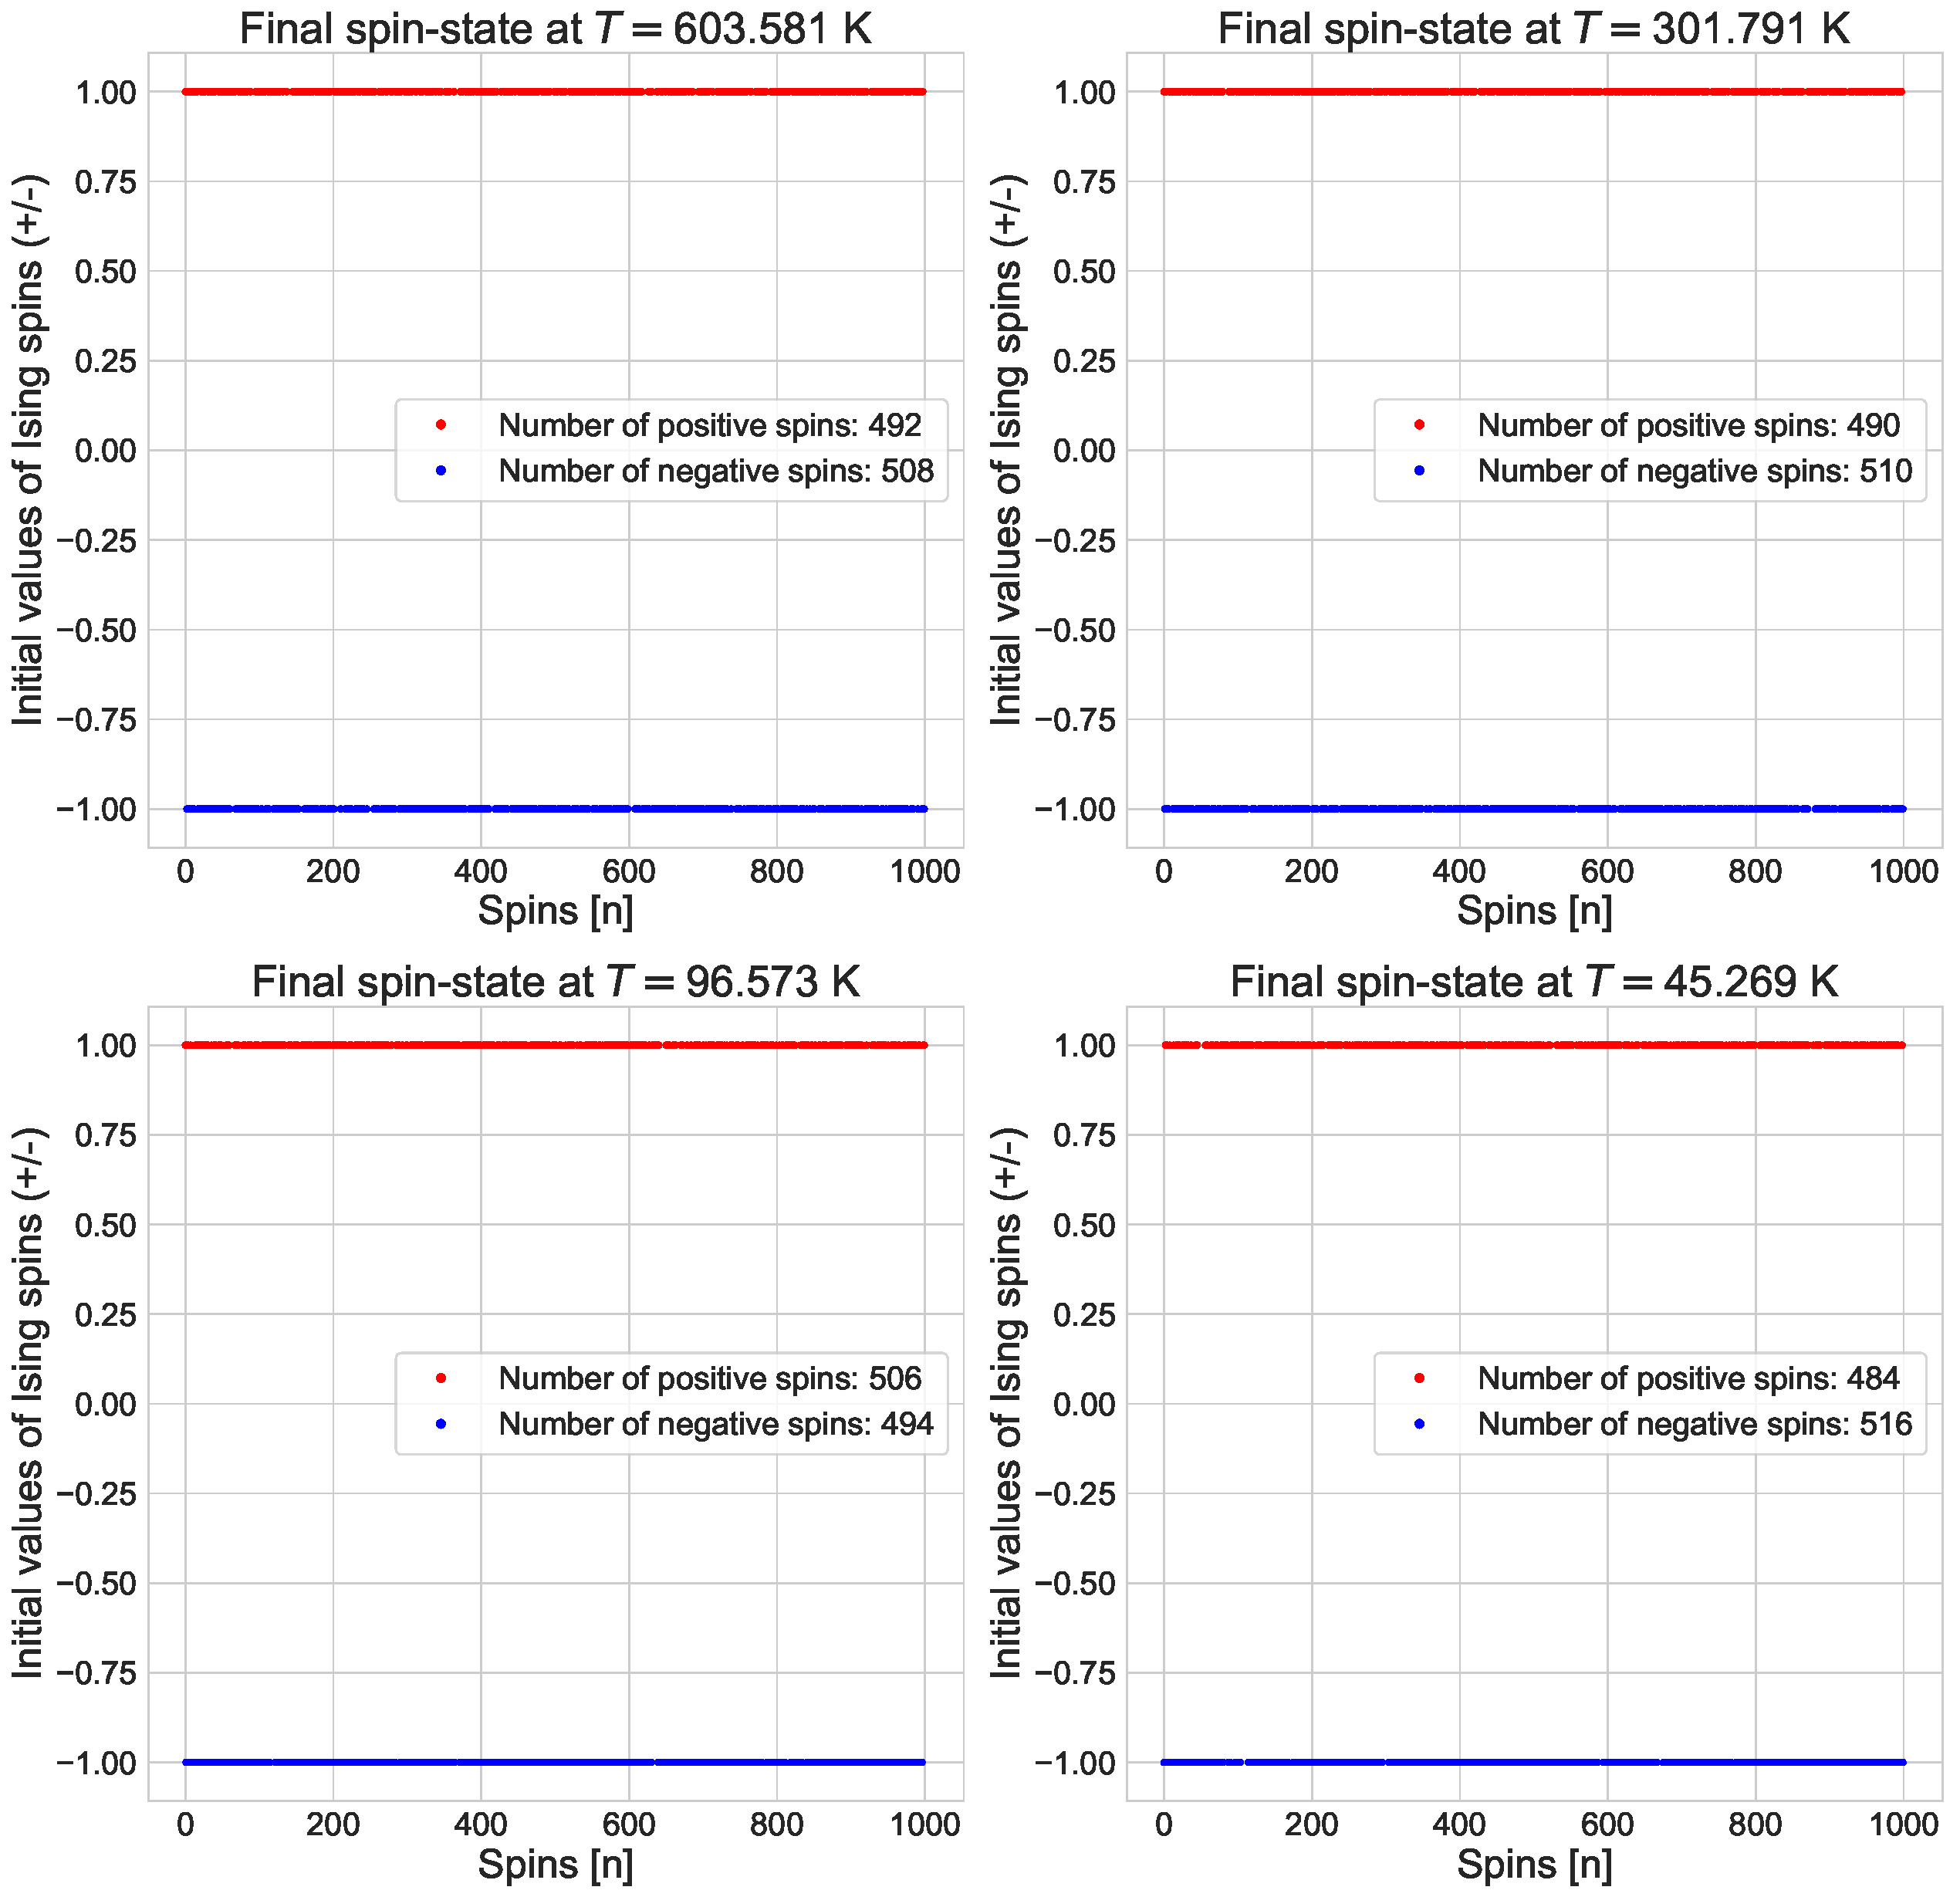
\includegraphics[width=\textwidth]{images/spin_states_1D.pdf}}
\captionof{figure}{Az 1D Ising-modell végső állapota $N=200\,000$ lépés szimulálása után} \label{fig:1}
\newpage
{\centering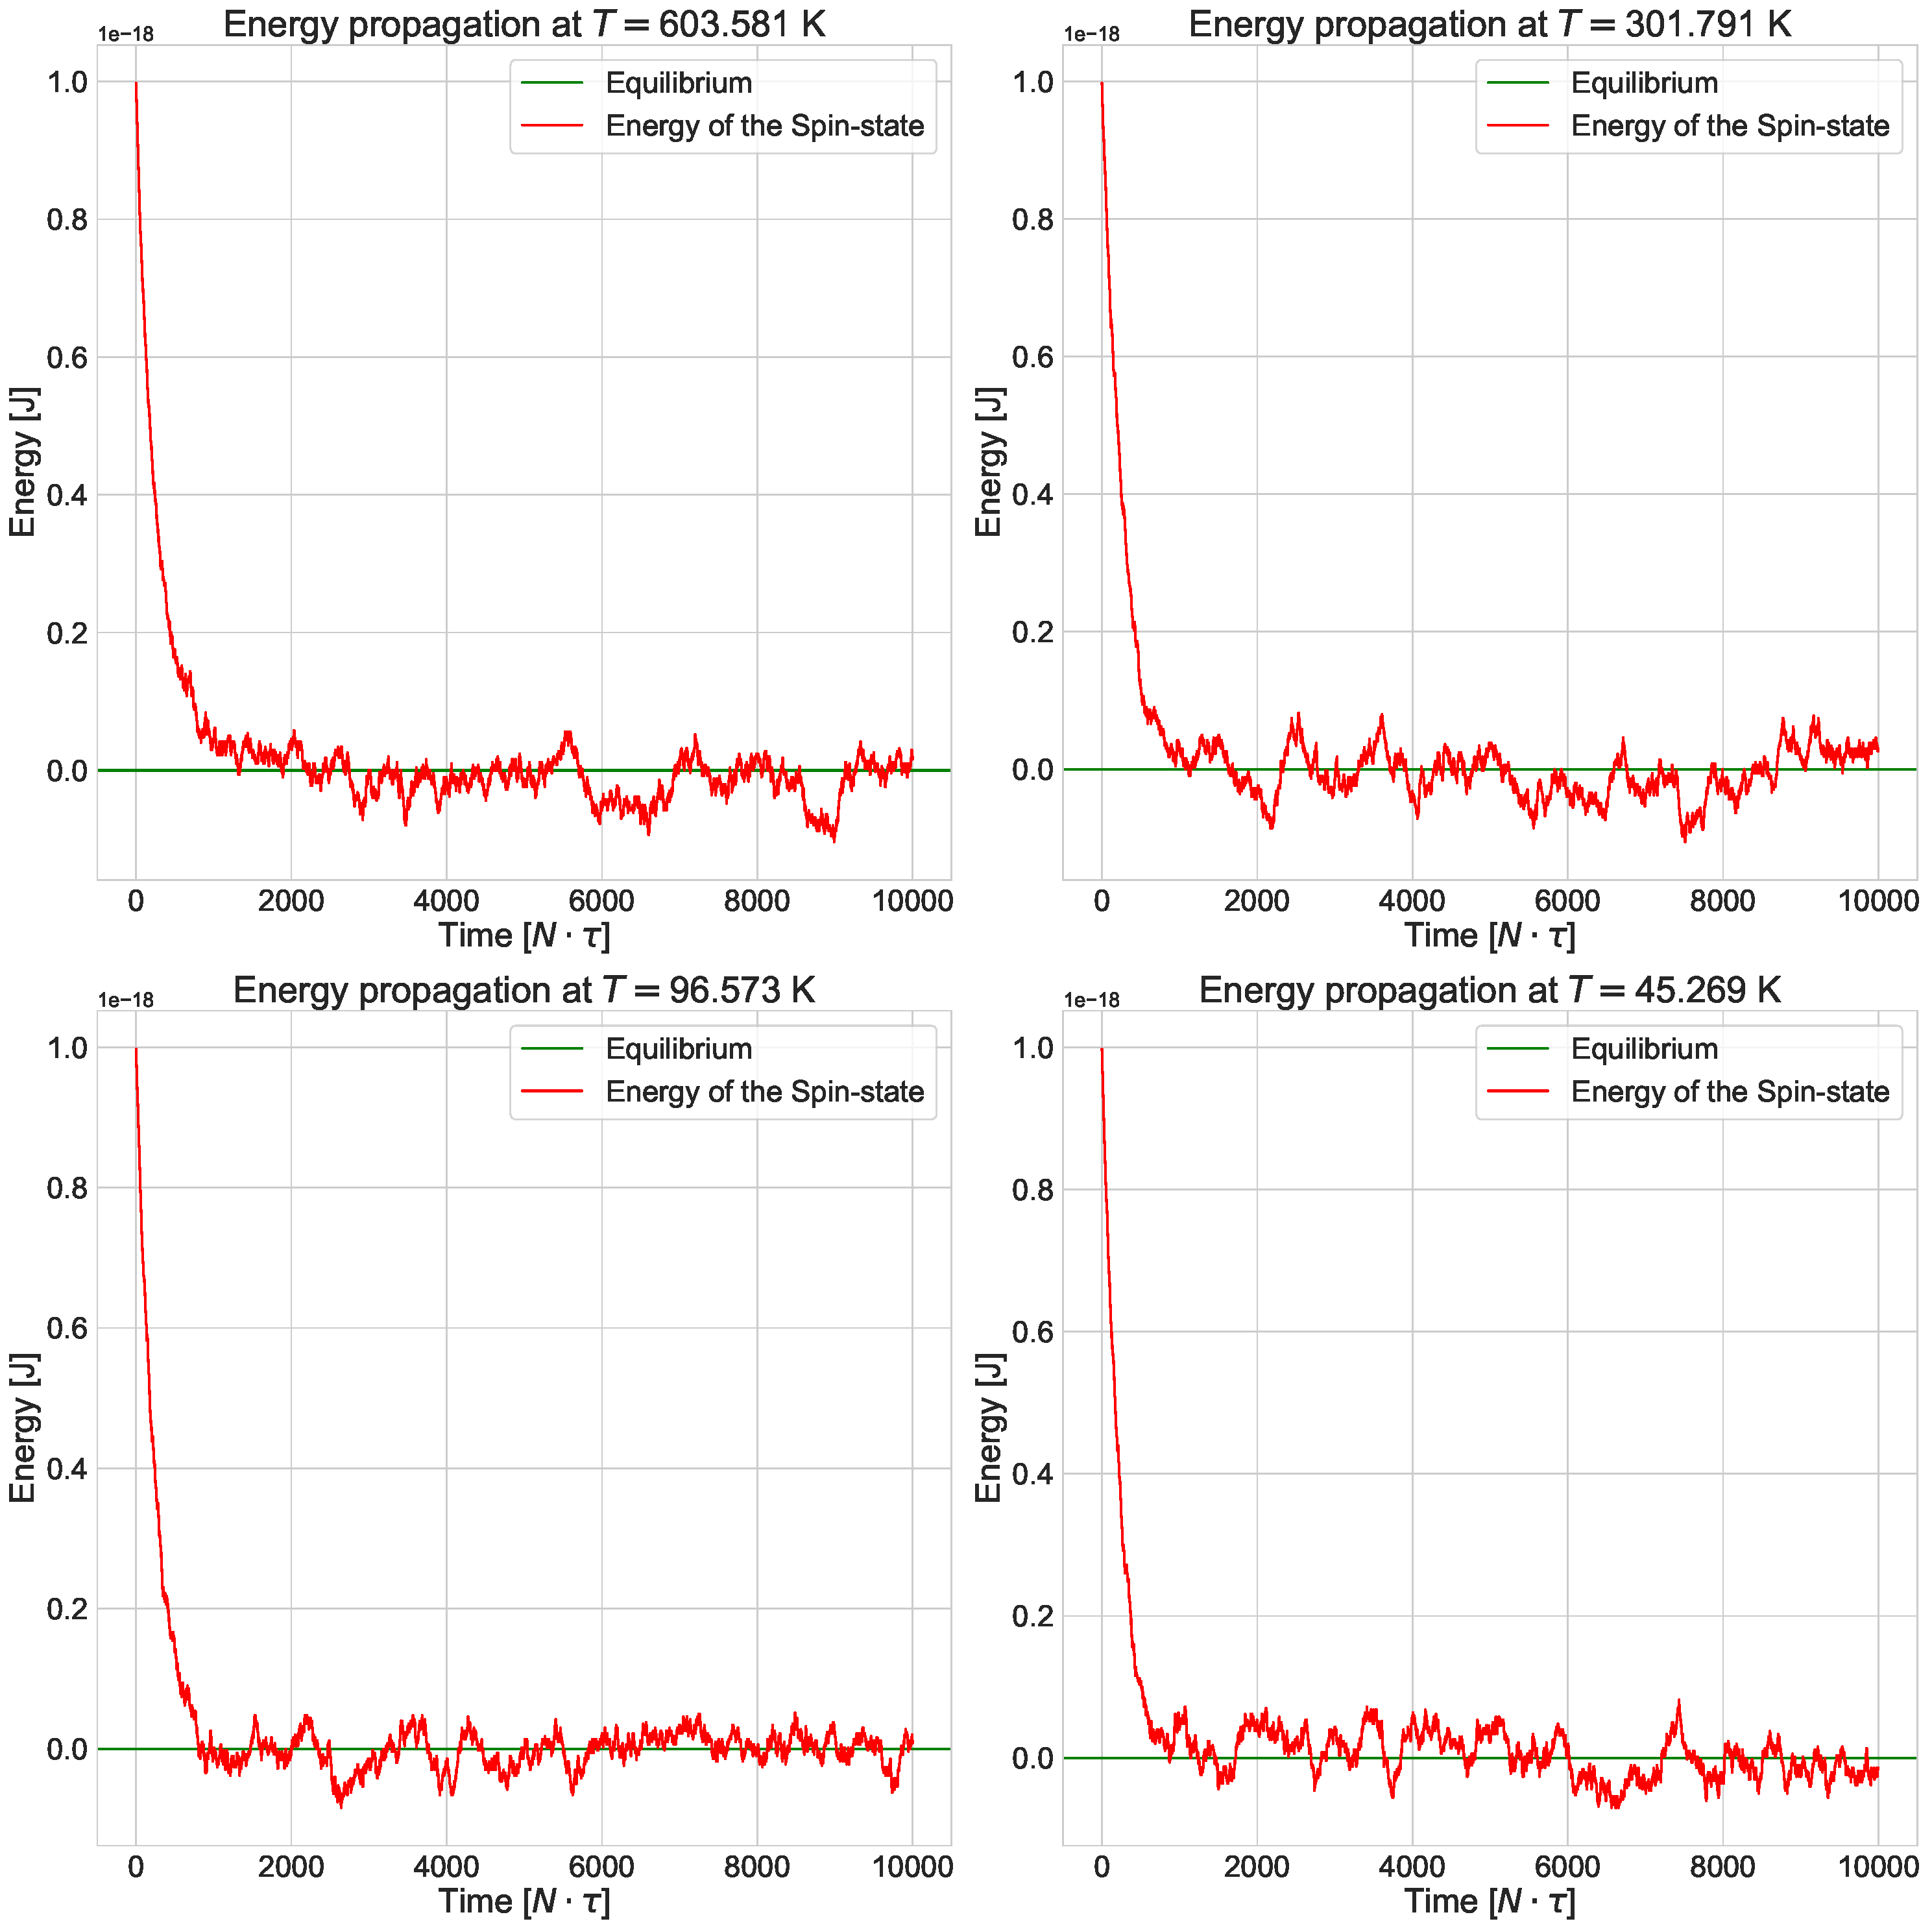
\includegraphics[width=\textwidth]{images/discrete_energies_1D.pdf}}
\captionof{figure}{Az 1D Ising-modellben mérhető teljes energia időfejlődése} \label{fig:2}
\newpage
{\centering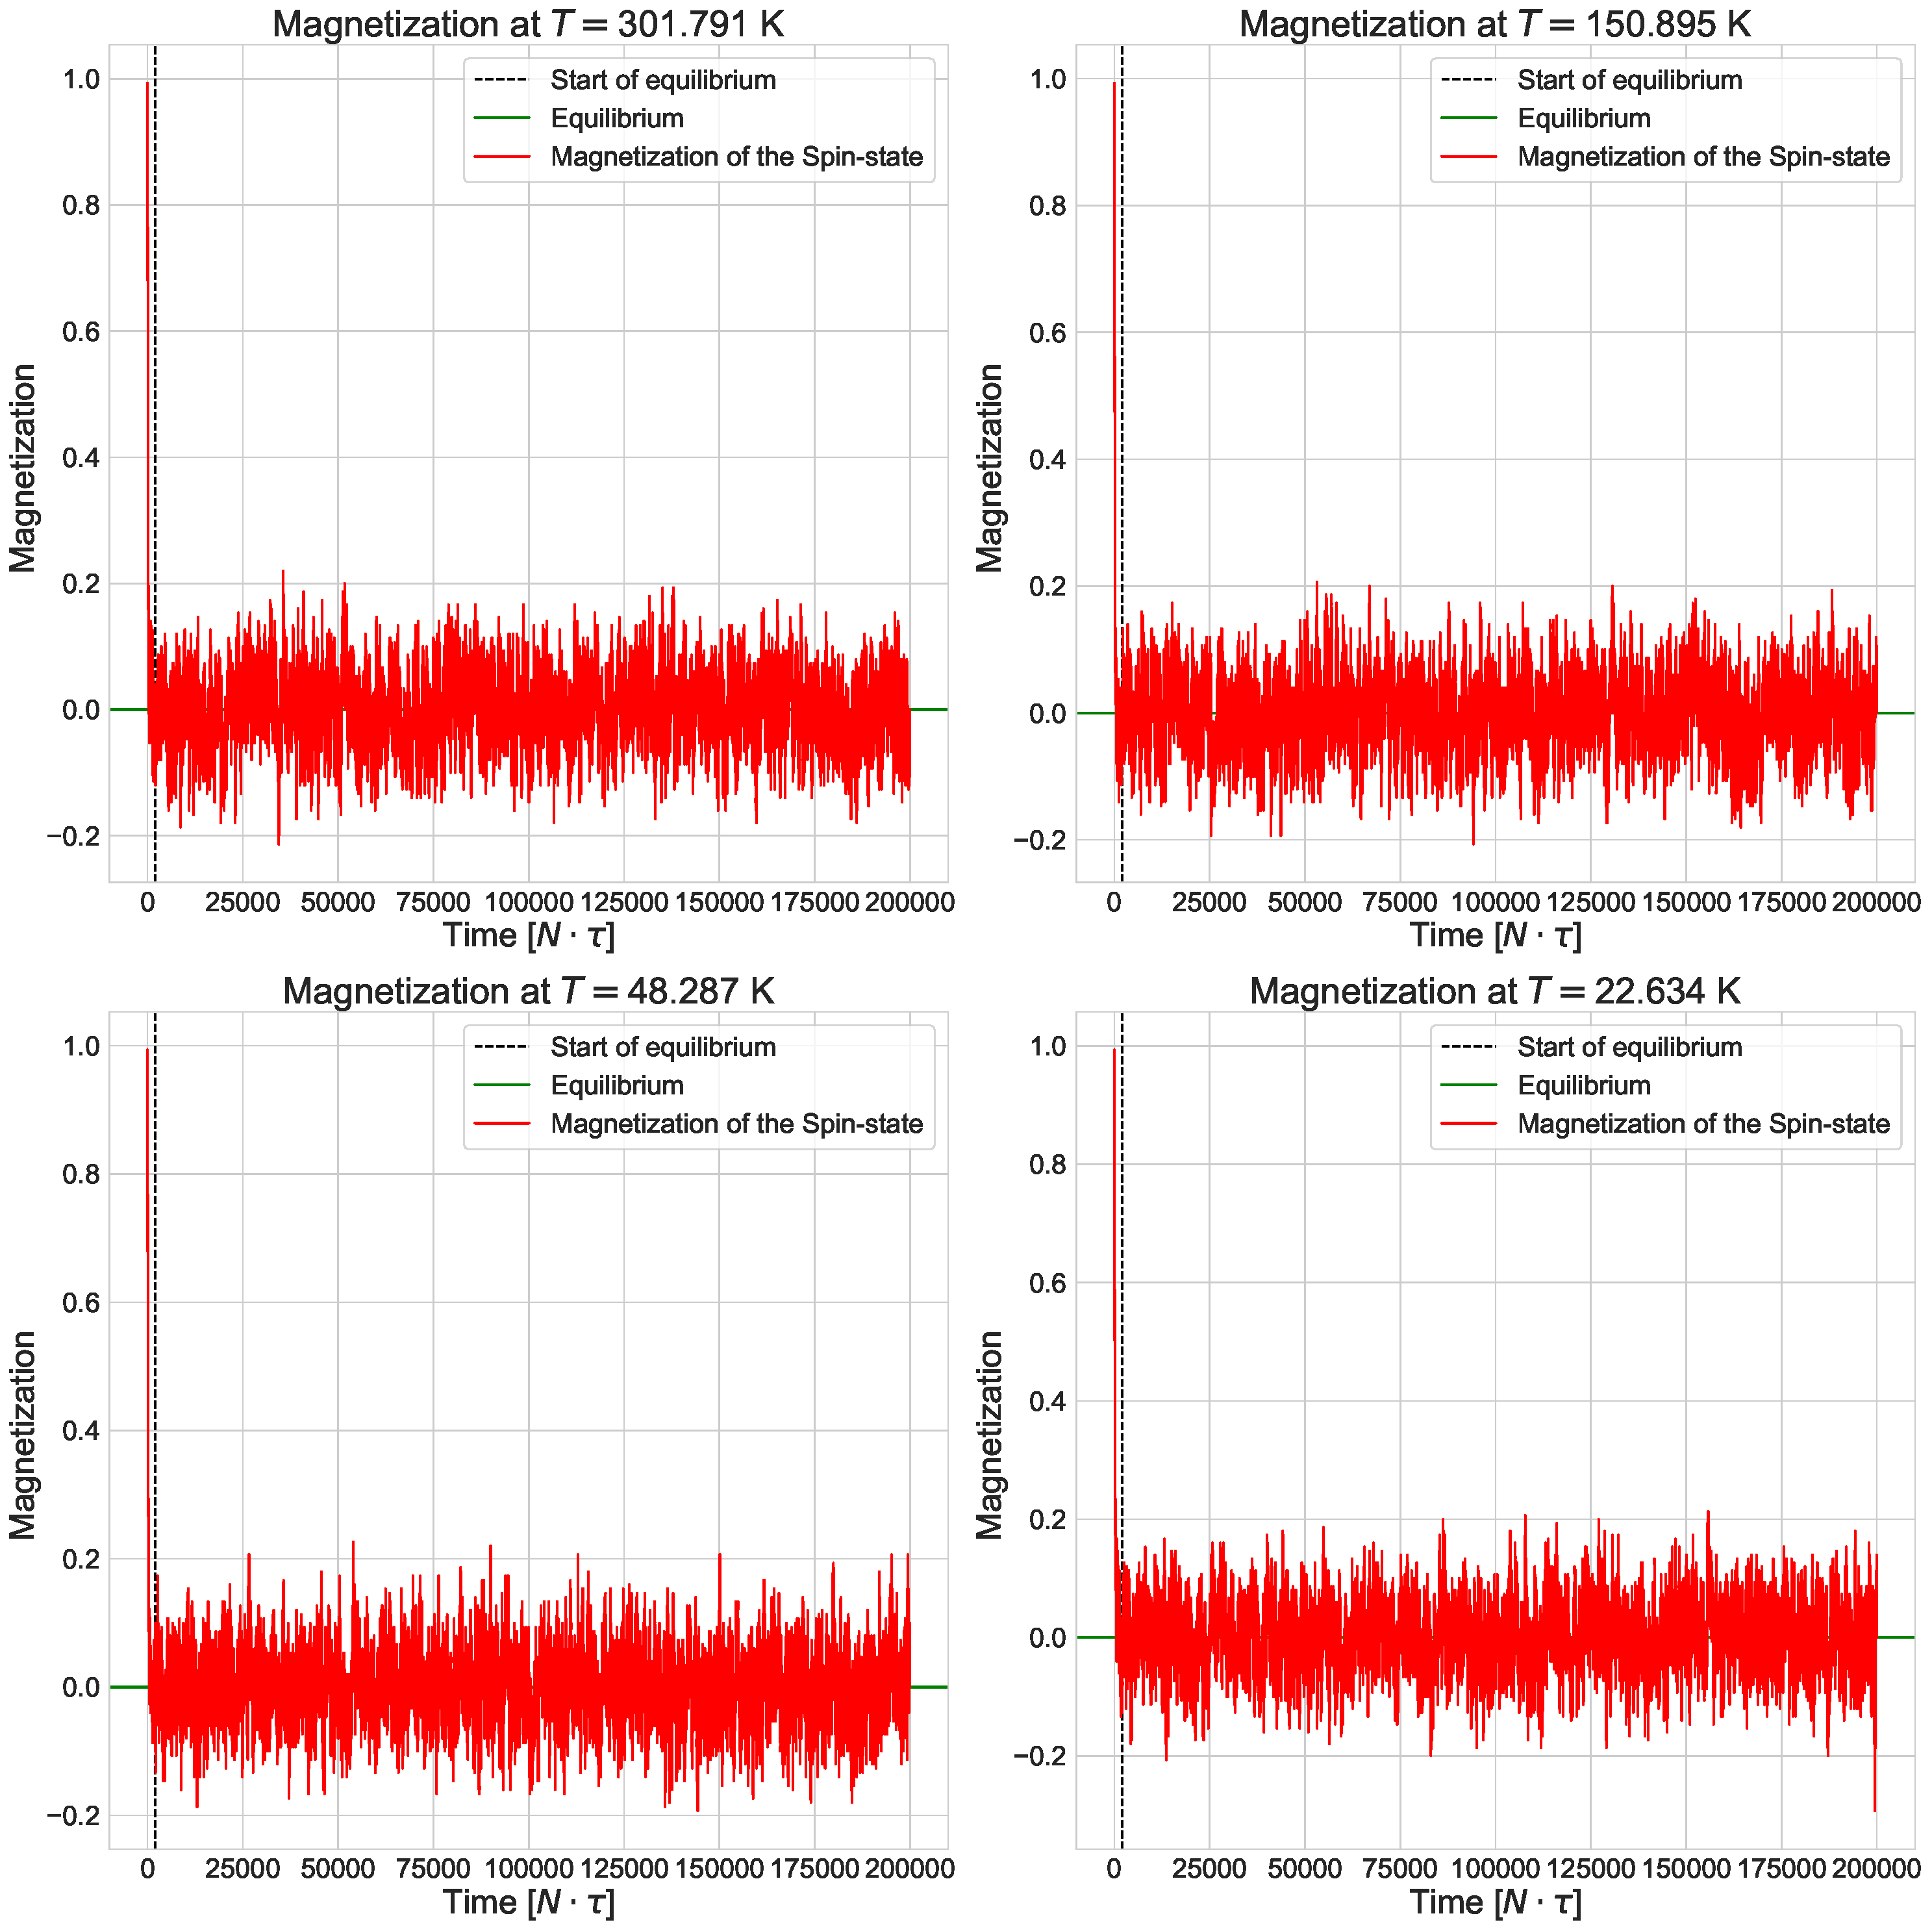
\includegraphics[width=\textwidth]{images/magnetization_1D.pdf}}
\captionof{figure}{Az 1D Ising-modellben mérhető mágnesezettség időfejlődése} \label{fig:3}
\newpage
{\centering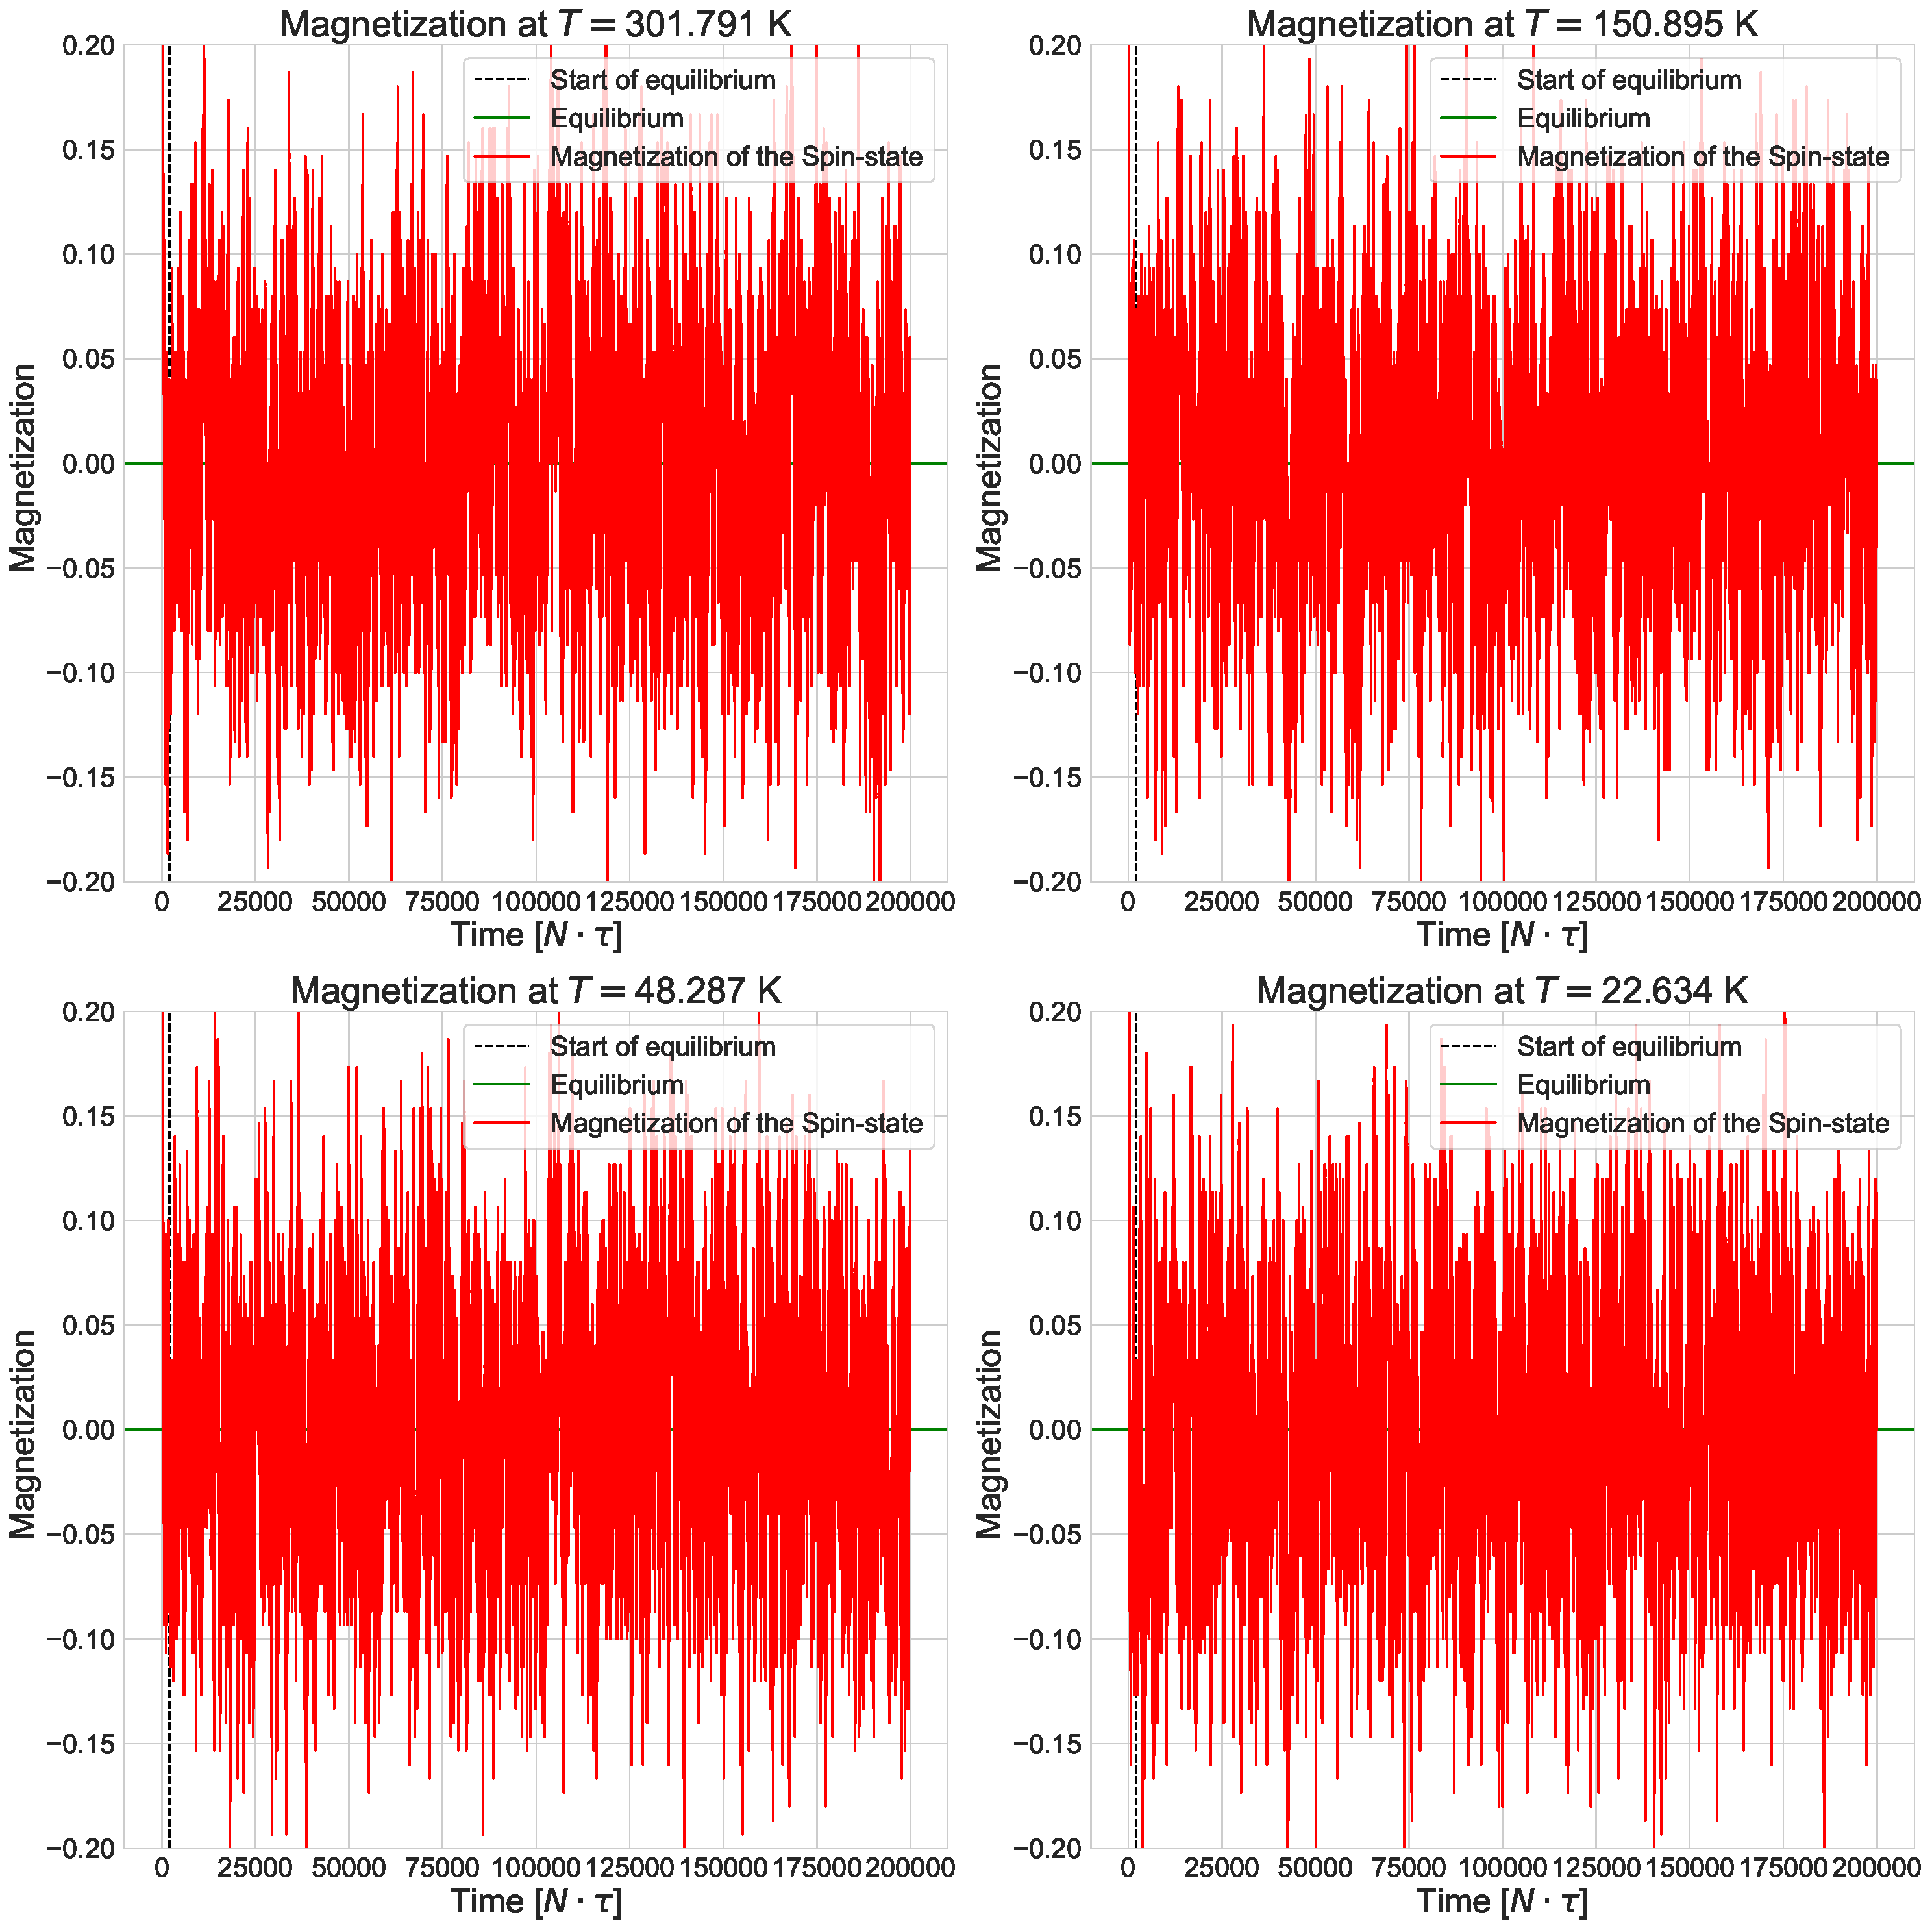
\includegraphics[width=\textwidth]{images/magnetization_1D_zoomed.pdf}}
\captionof{figure}{Az 1D Ising-modellben mérhető mágnesezettség időfejlődése -- Kiemelt fluktuáció} \label{fig:4}
\newpage
{\centering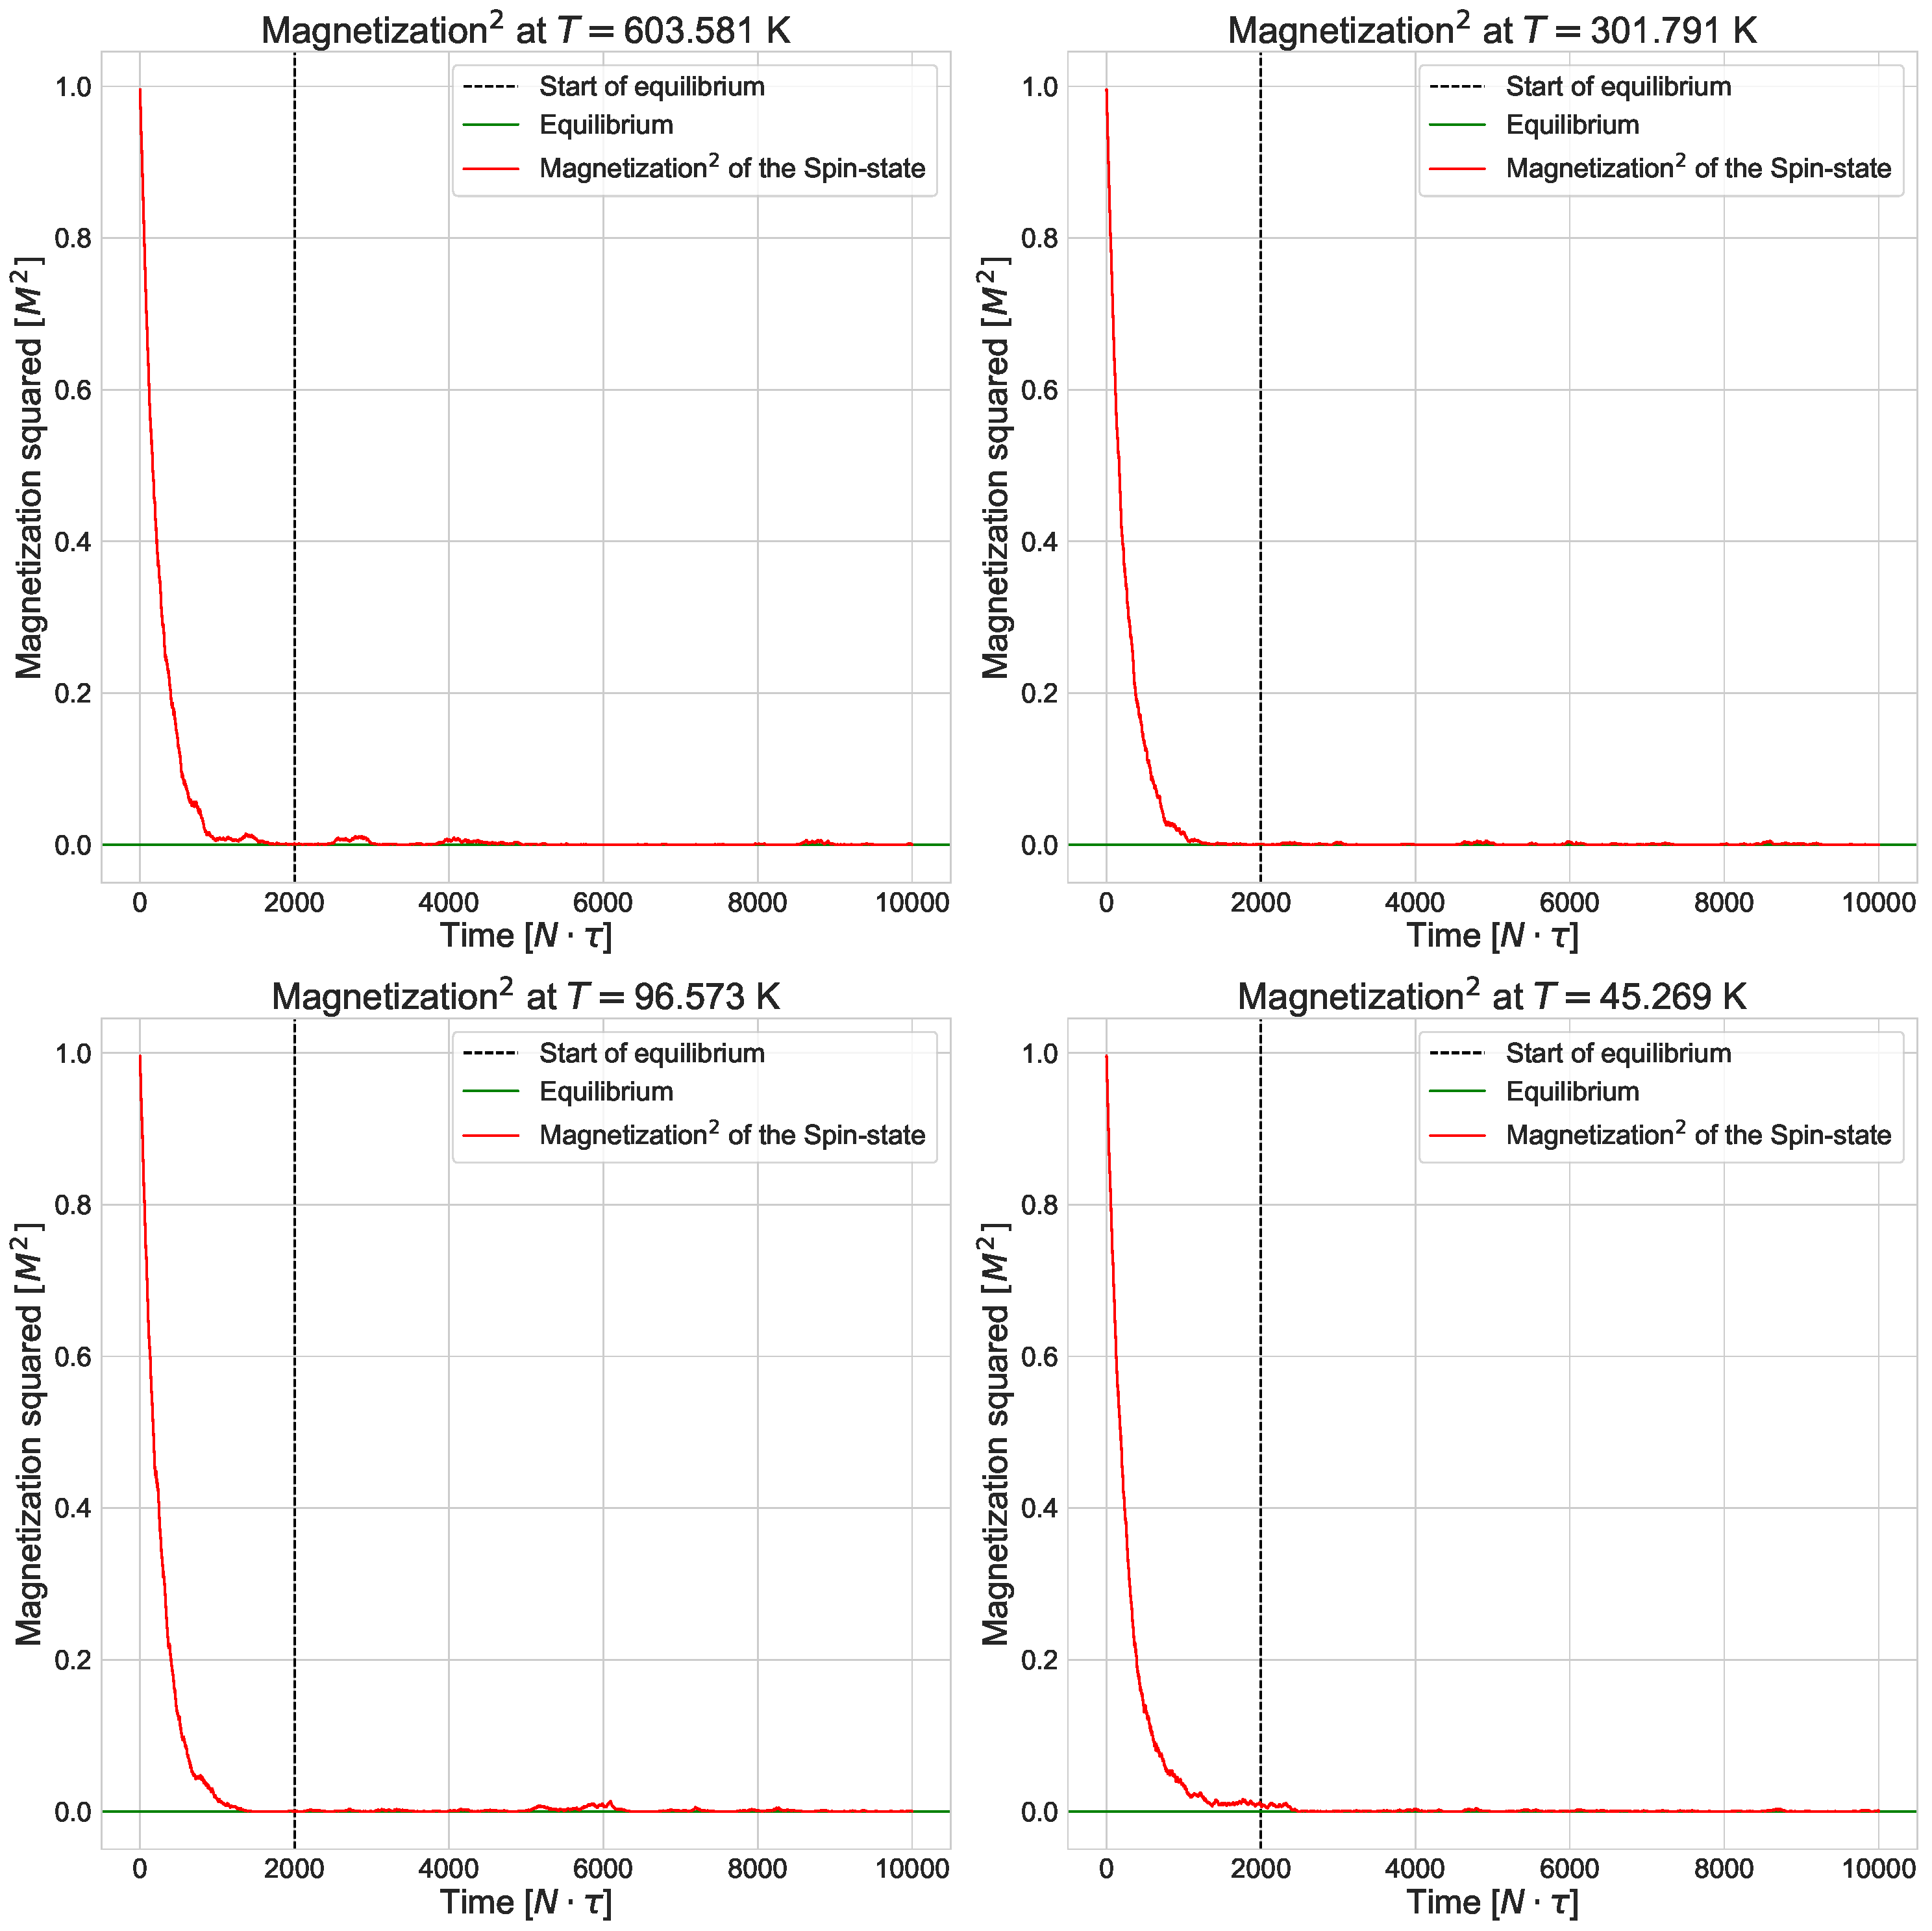
\includegraphics[width=\textwidth]{images/magnetization_squared_1D.pdf}}
\captionof{figure}{Az 1D Ising-modellben mérhető mágnesezettség négyzetének időfejlődése} \label{fig:5}
\newpage
{\centering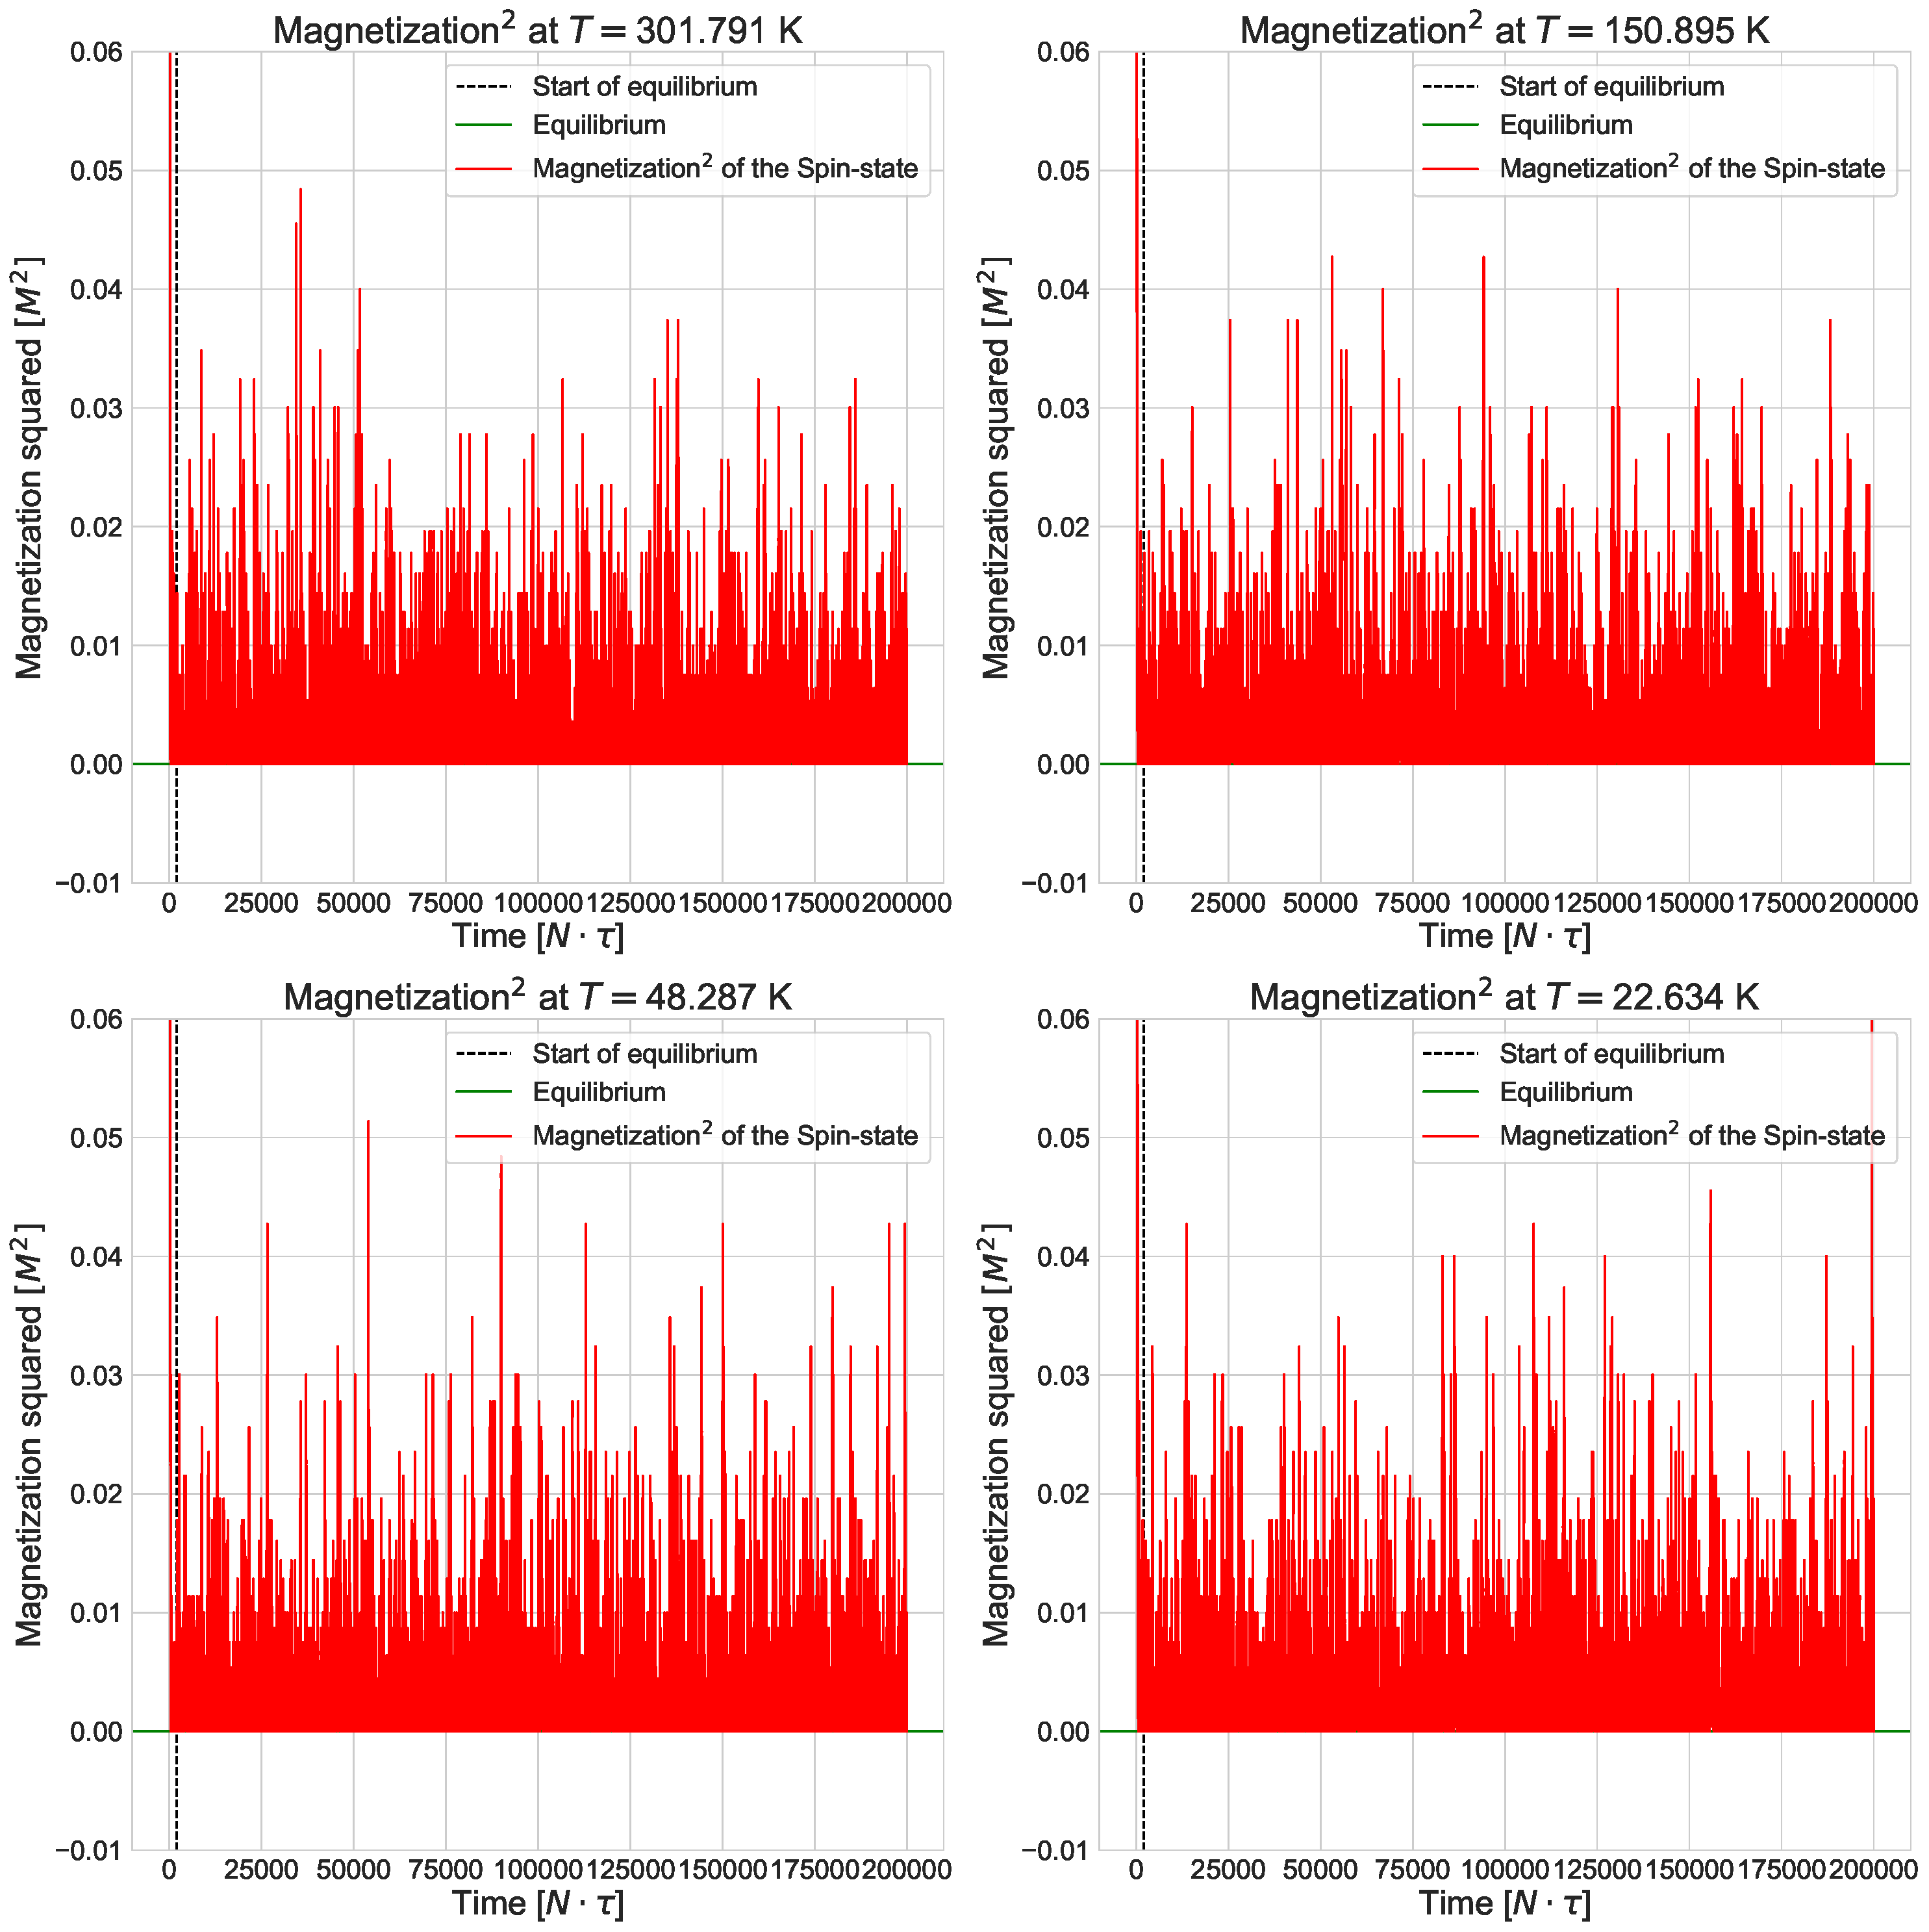
\includegraphics[width=\textwidth]{images/magnetization_squared_1D_zoomed.pdf}}
\captionof{figure}{Az 1D Ising-modellben mérhető mágnesezettség négyzetének időfejlődése -- Kiemelt fluktuáció} \label{fig:6}
\newpage
{\centering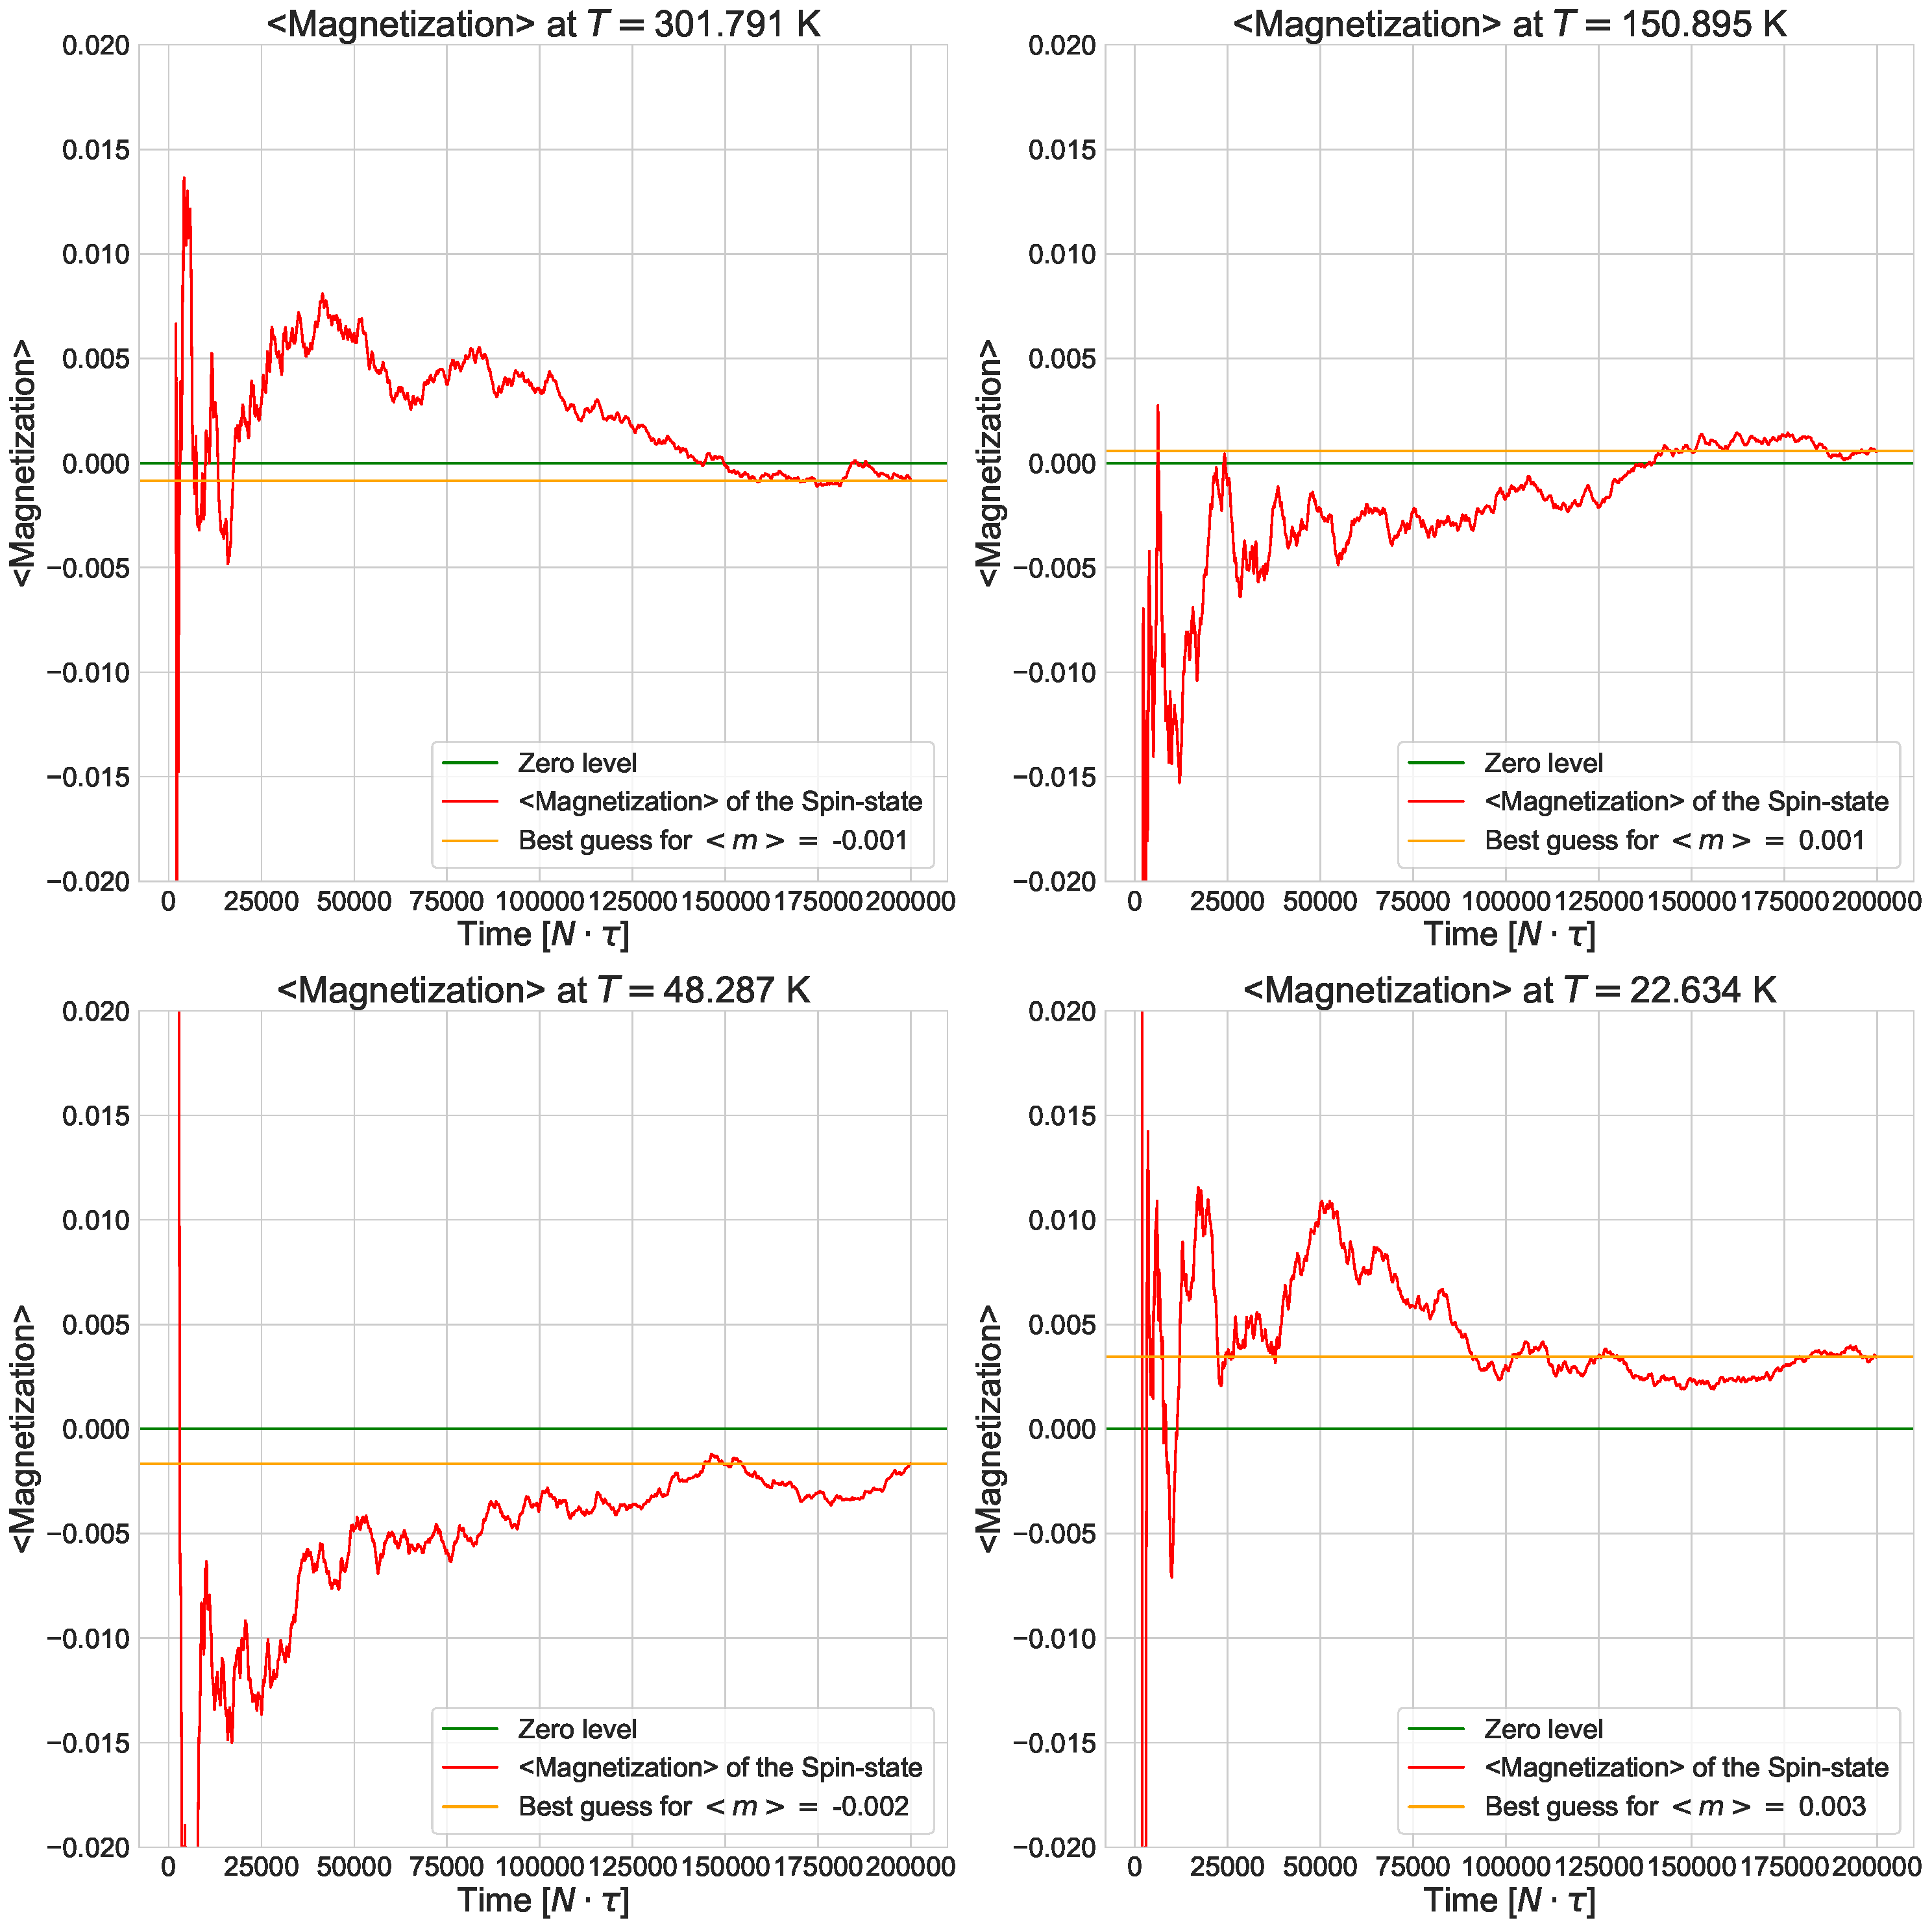
\includegraphics[width=\textwidth]{images/magnetization_mean_1D_off2000.pdf}}
\captionof{figure}{Az 1D Ising-modellben az egyensúlyi helyzet beállta után mérhető mágnesezettség időátlaga} \label{fig:7}
\newpage
{\centering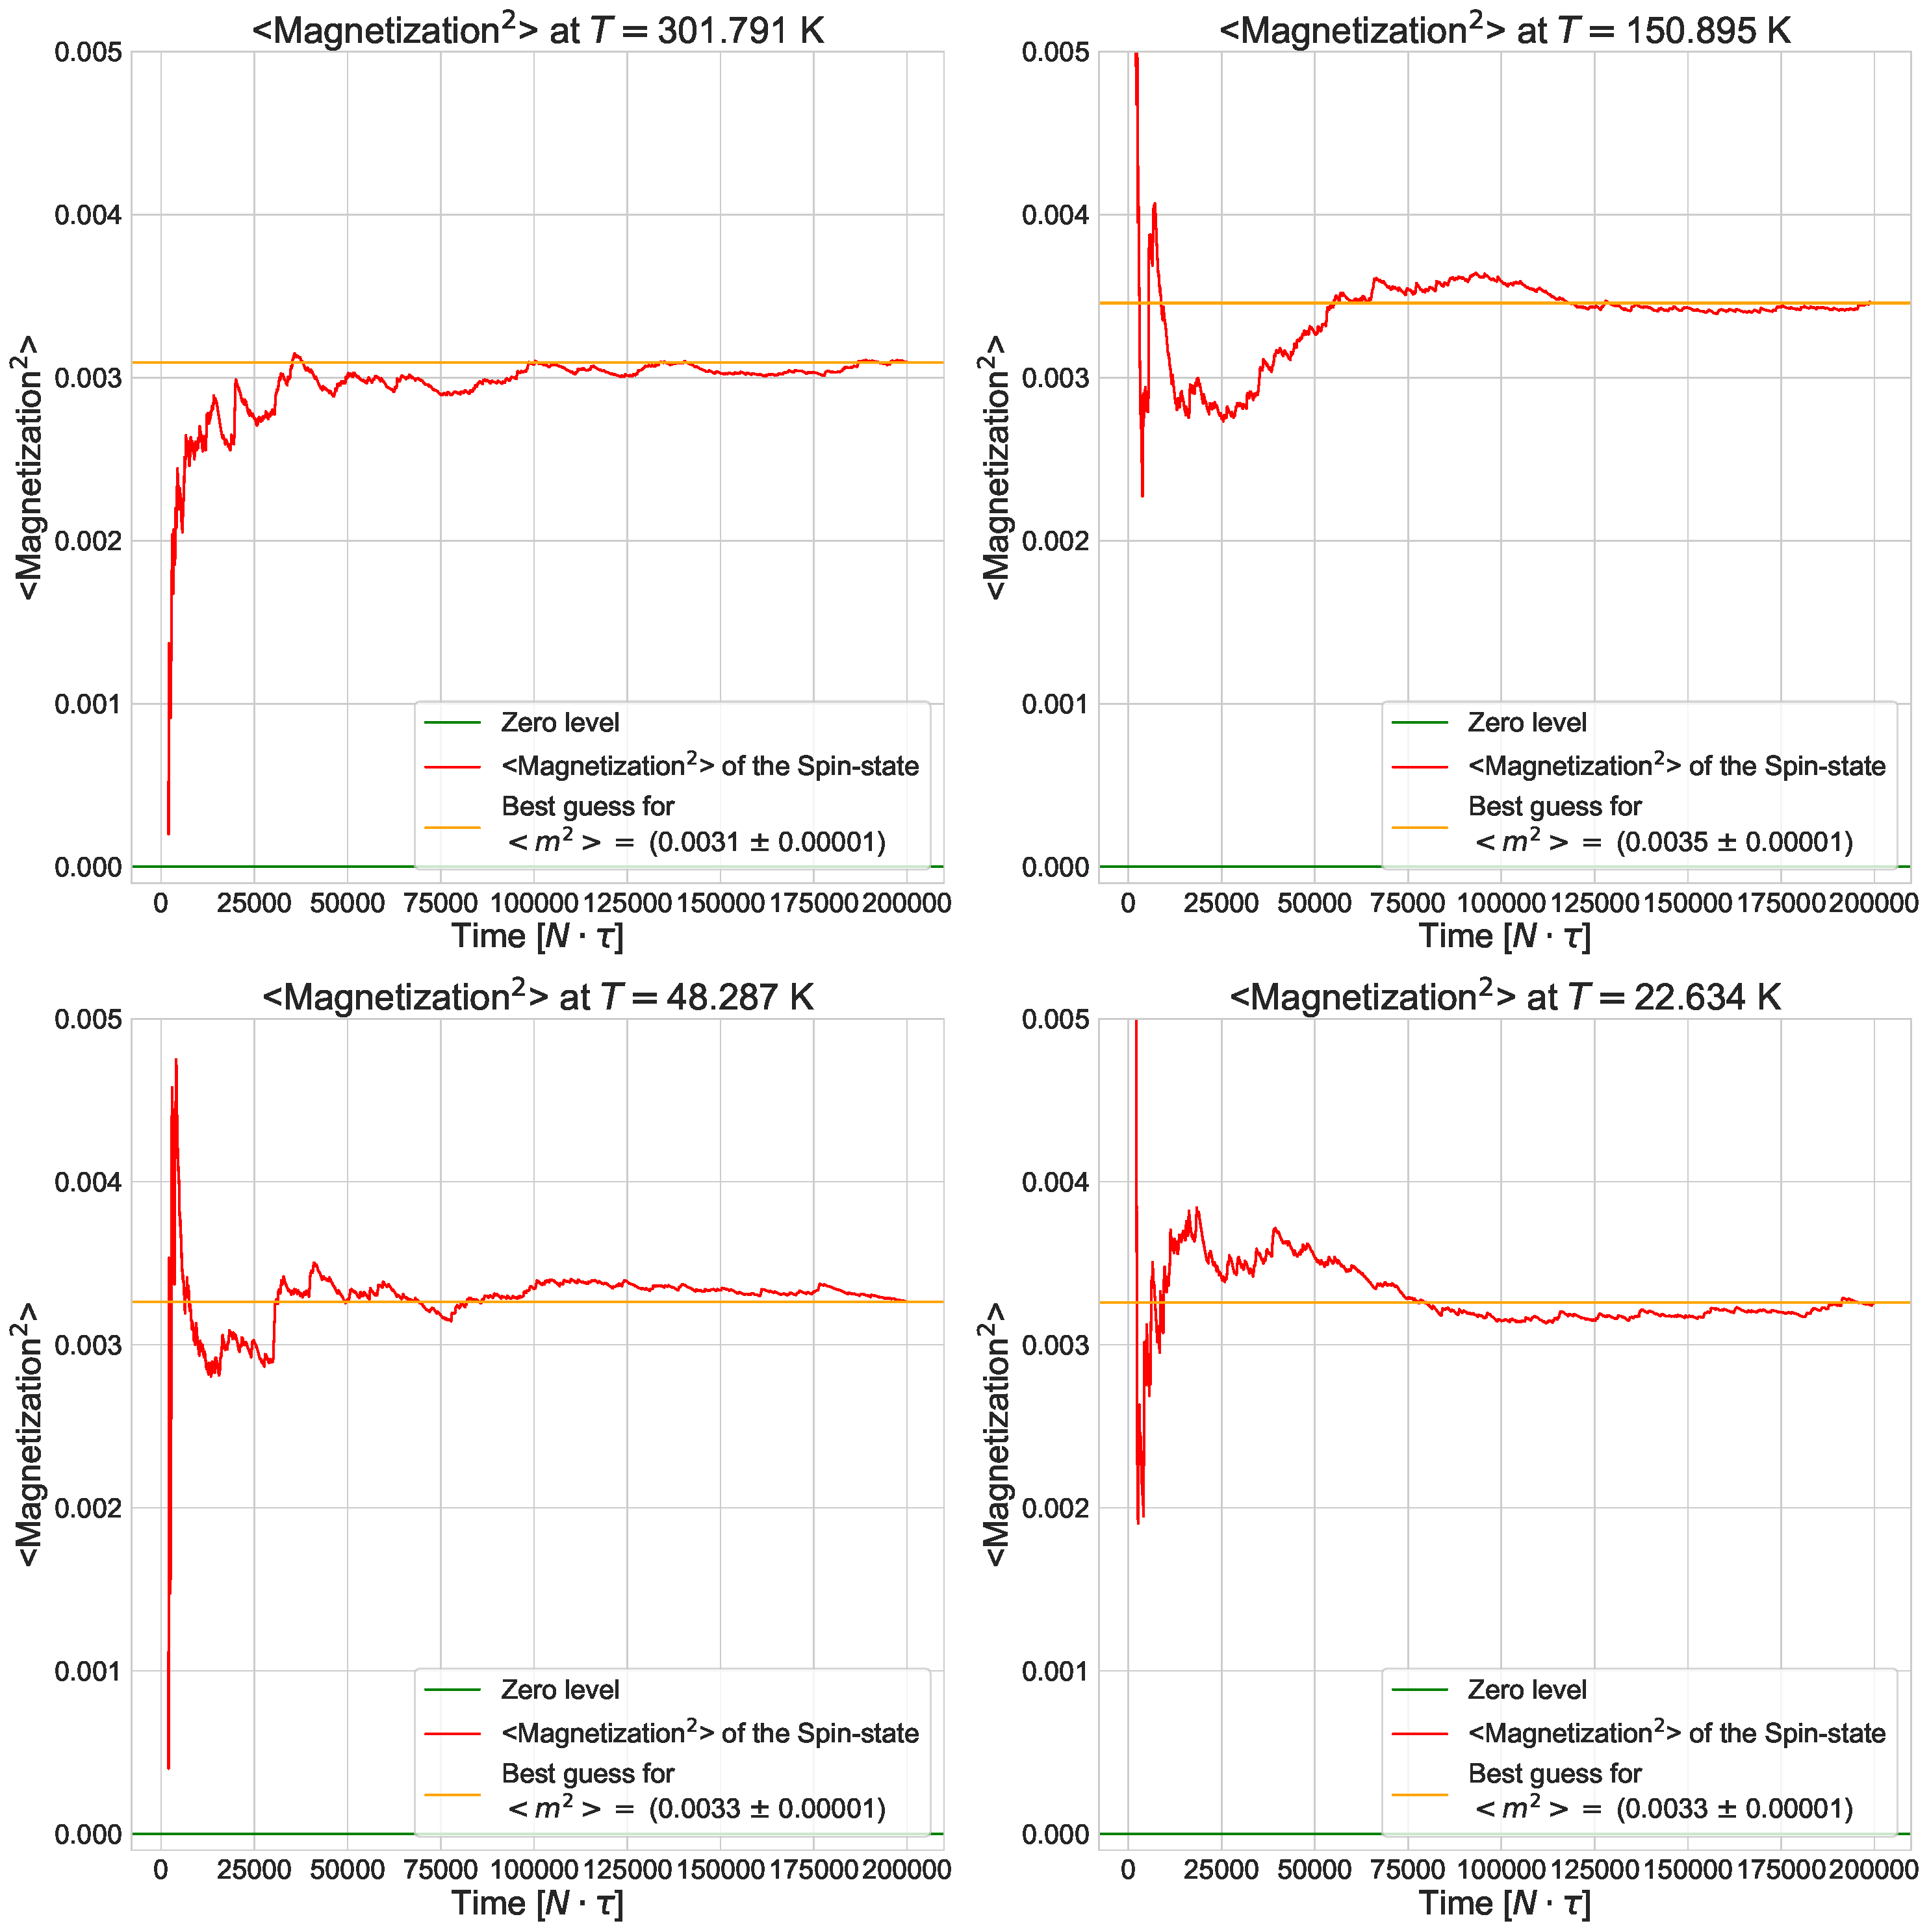
\includegraphics[width=\textwidth]{images/magnetization_squared_mean_1D_off2000.pdf}}
\captionof{figure}{Az 1D Ising-modellben az egyensúlyi helyzet beállta után mérhető mágnesezettség négyzetének időátlaga} \label{fig:8}
\newpage
{\centering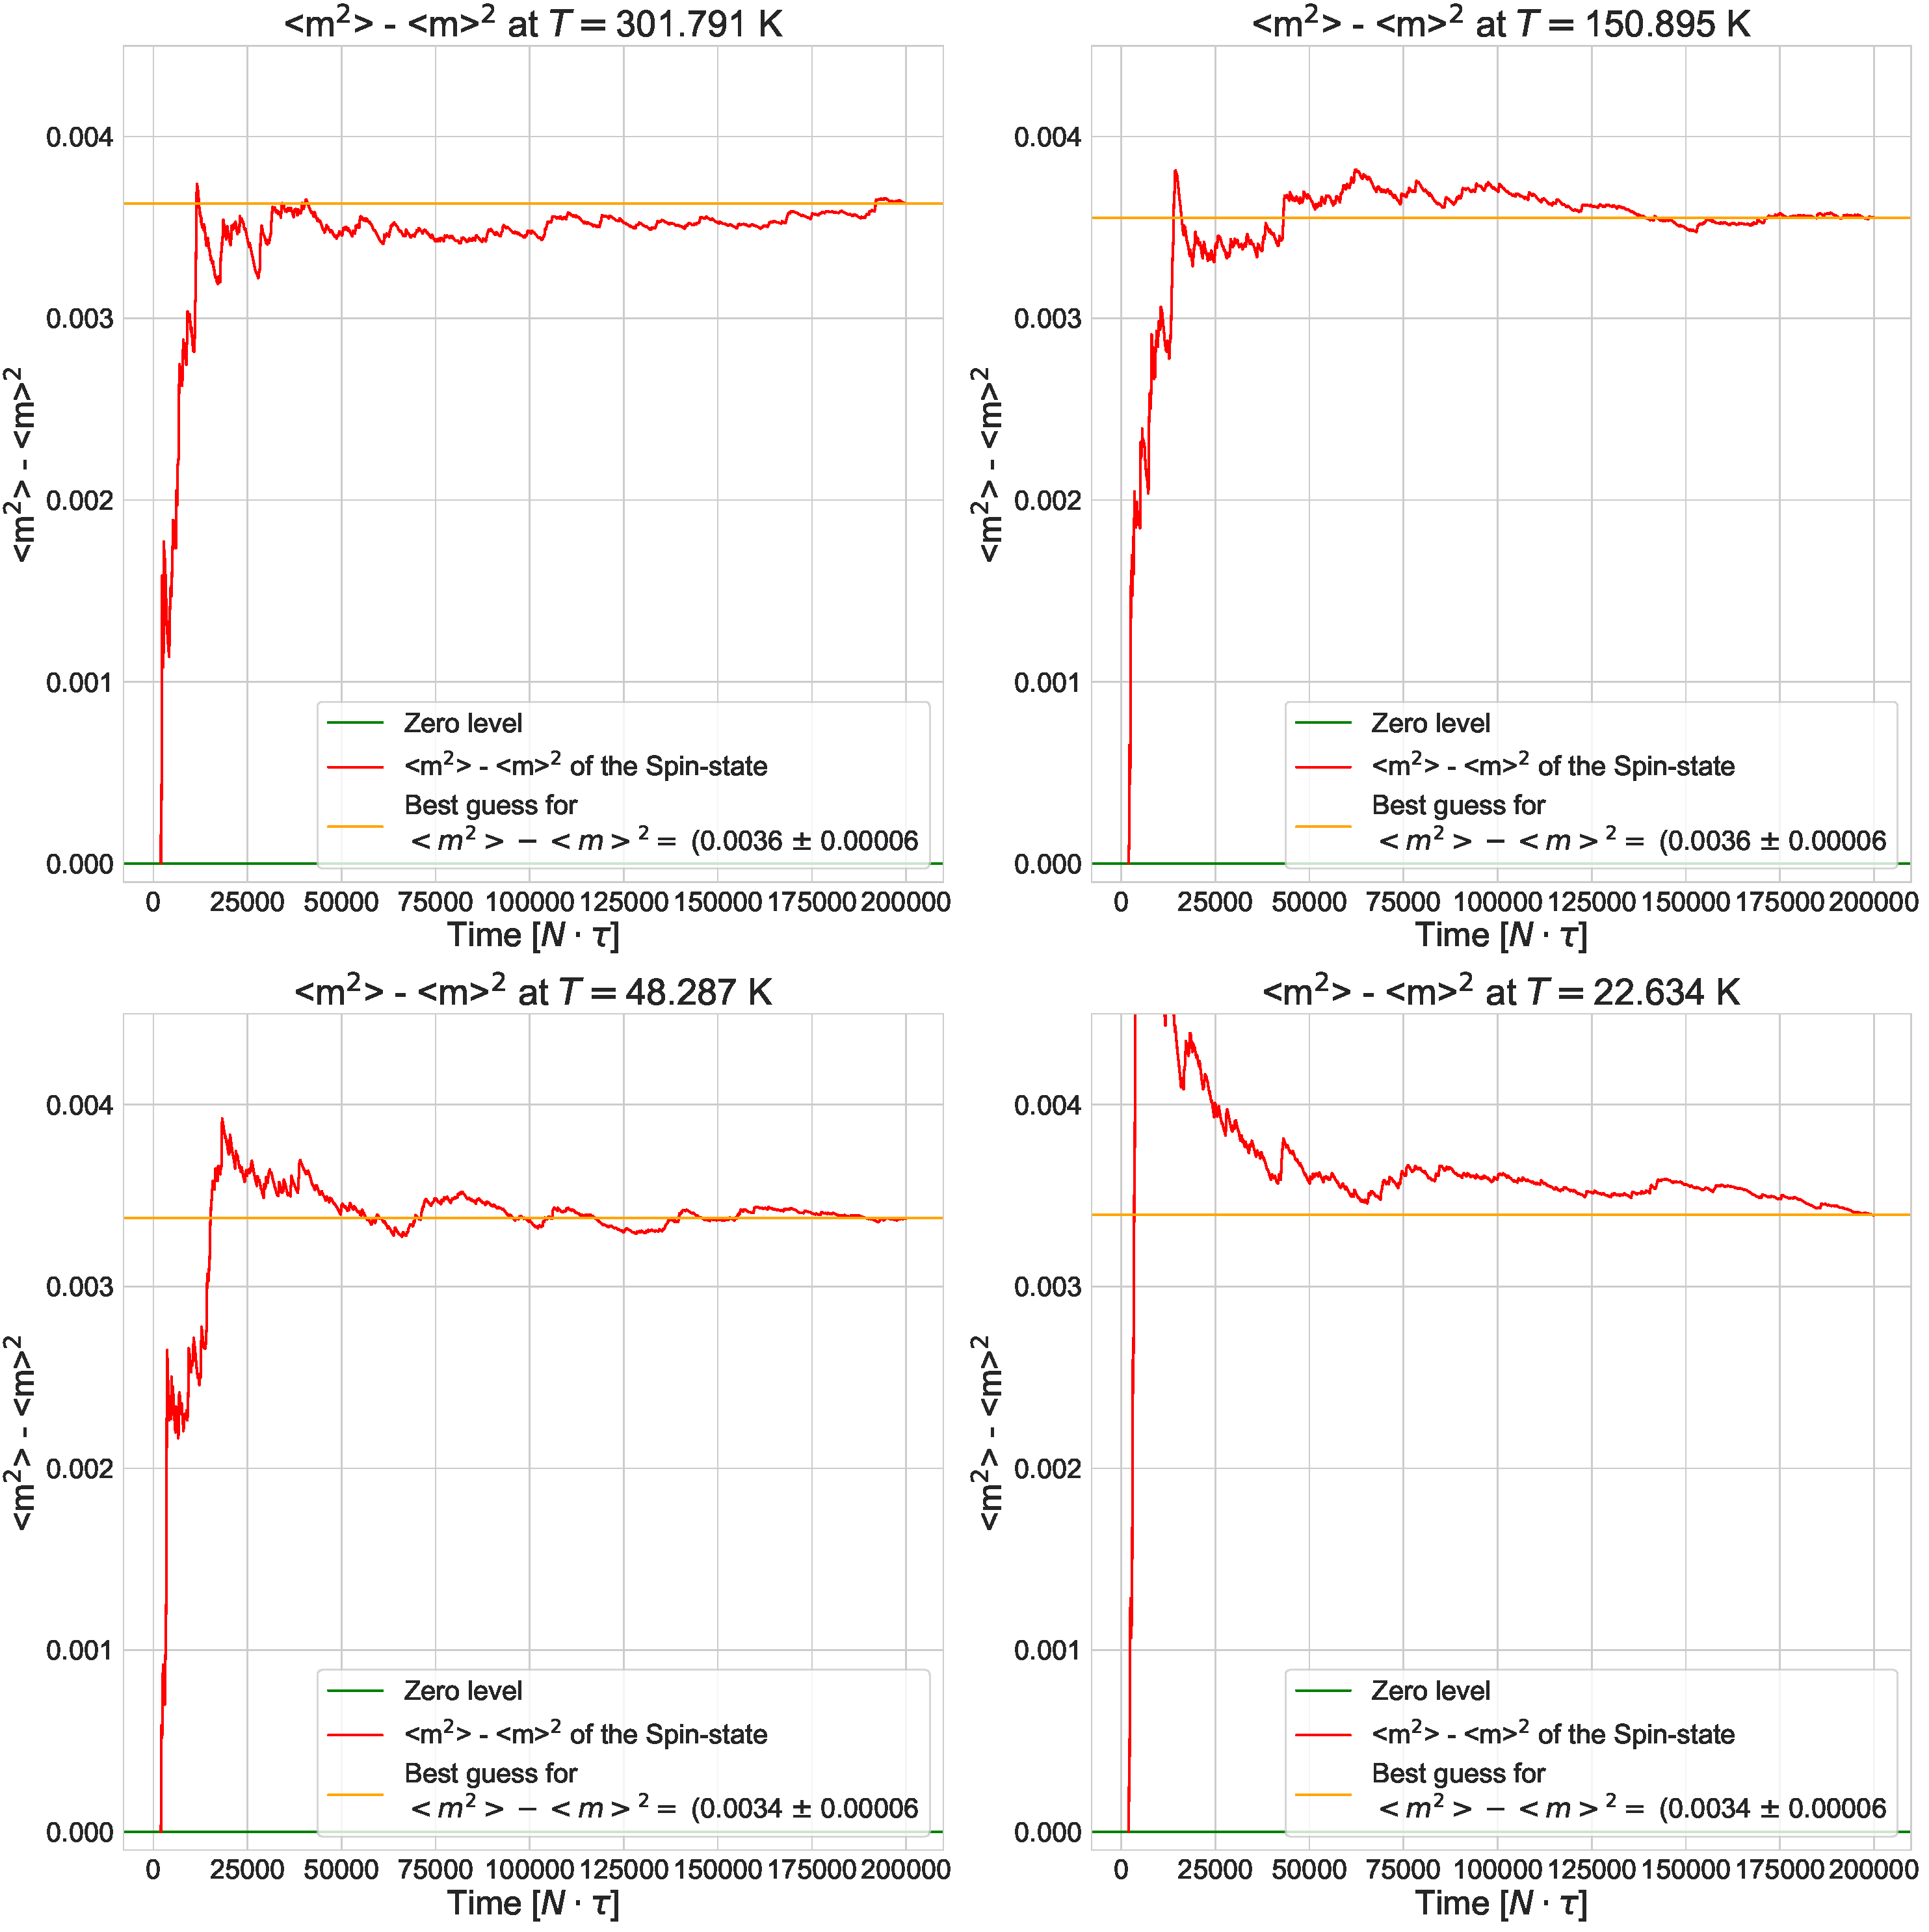
\includegraphics[width=\textwidth]{images/magnetization_diff_mean_1D_off2000.pdf}}
\captionof{figure}{Az 1D Ising-modellben az egyensúlyi helyzet beállta után mérhető $\left< m^{2} \right> - \left< m \right>^{2}$ mennyiség időátlaga} \label{fig:9}
\newpage


\subsection*{\bfseries\MakeUppercase{A.1\ \ A 2-dimenziós Ising-modell}} \label{A.1.2}
{\centering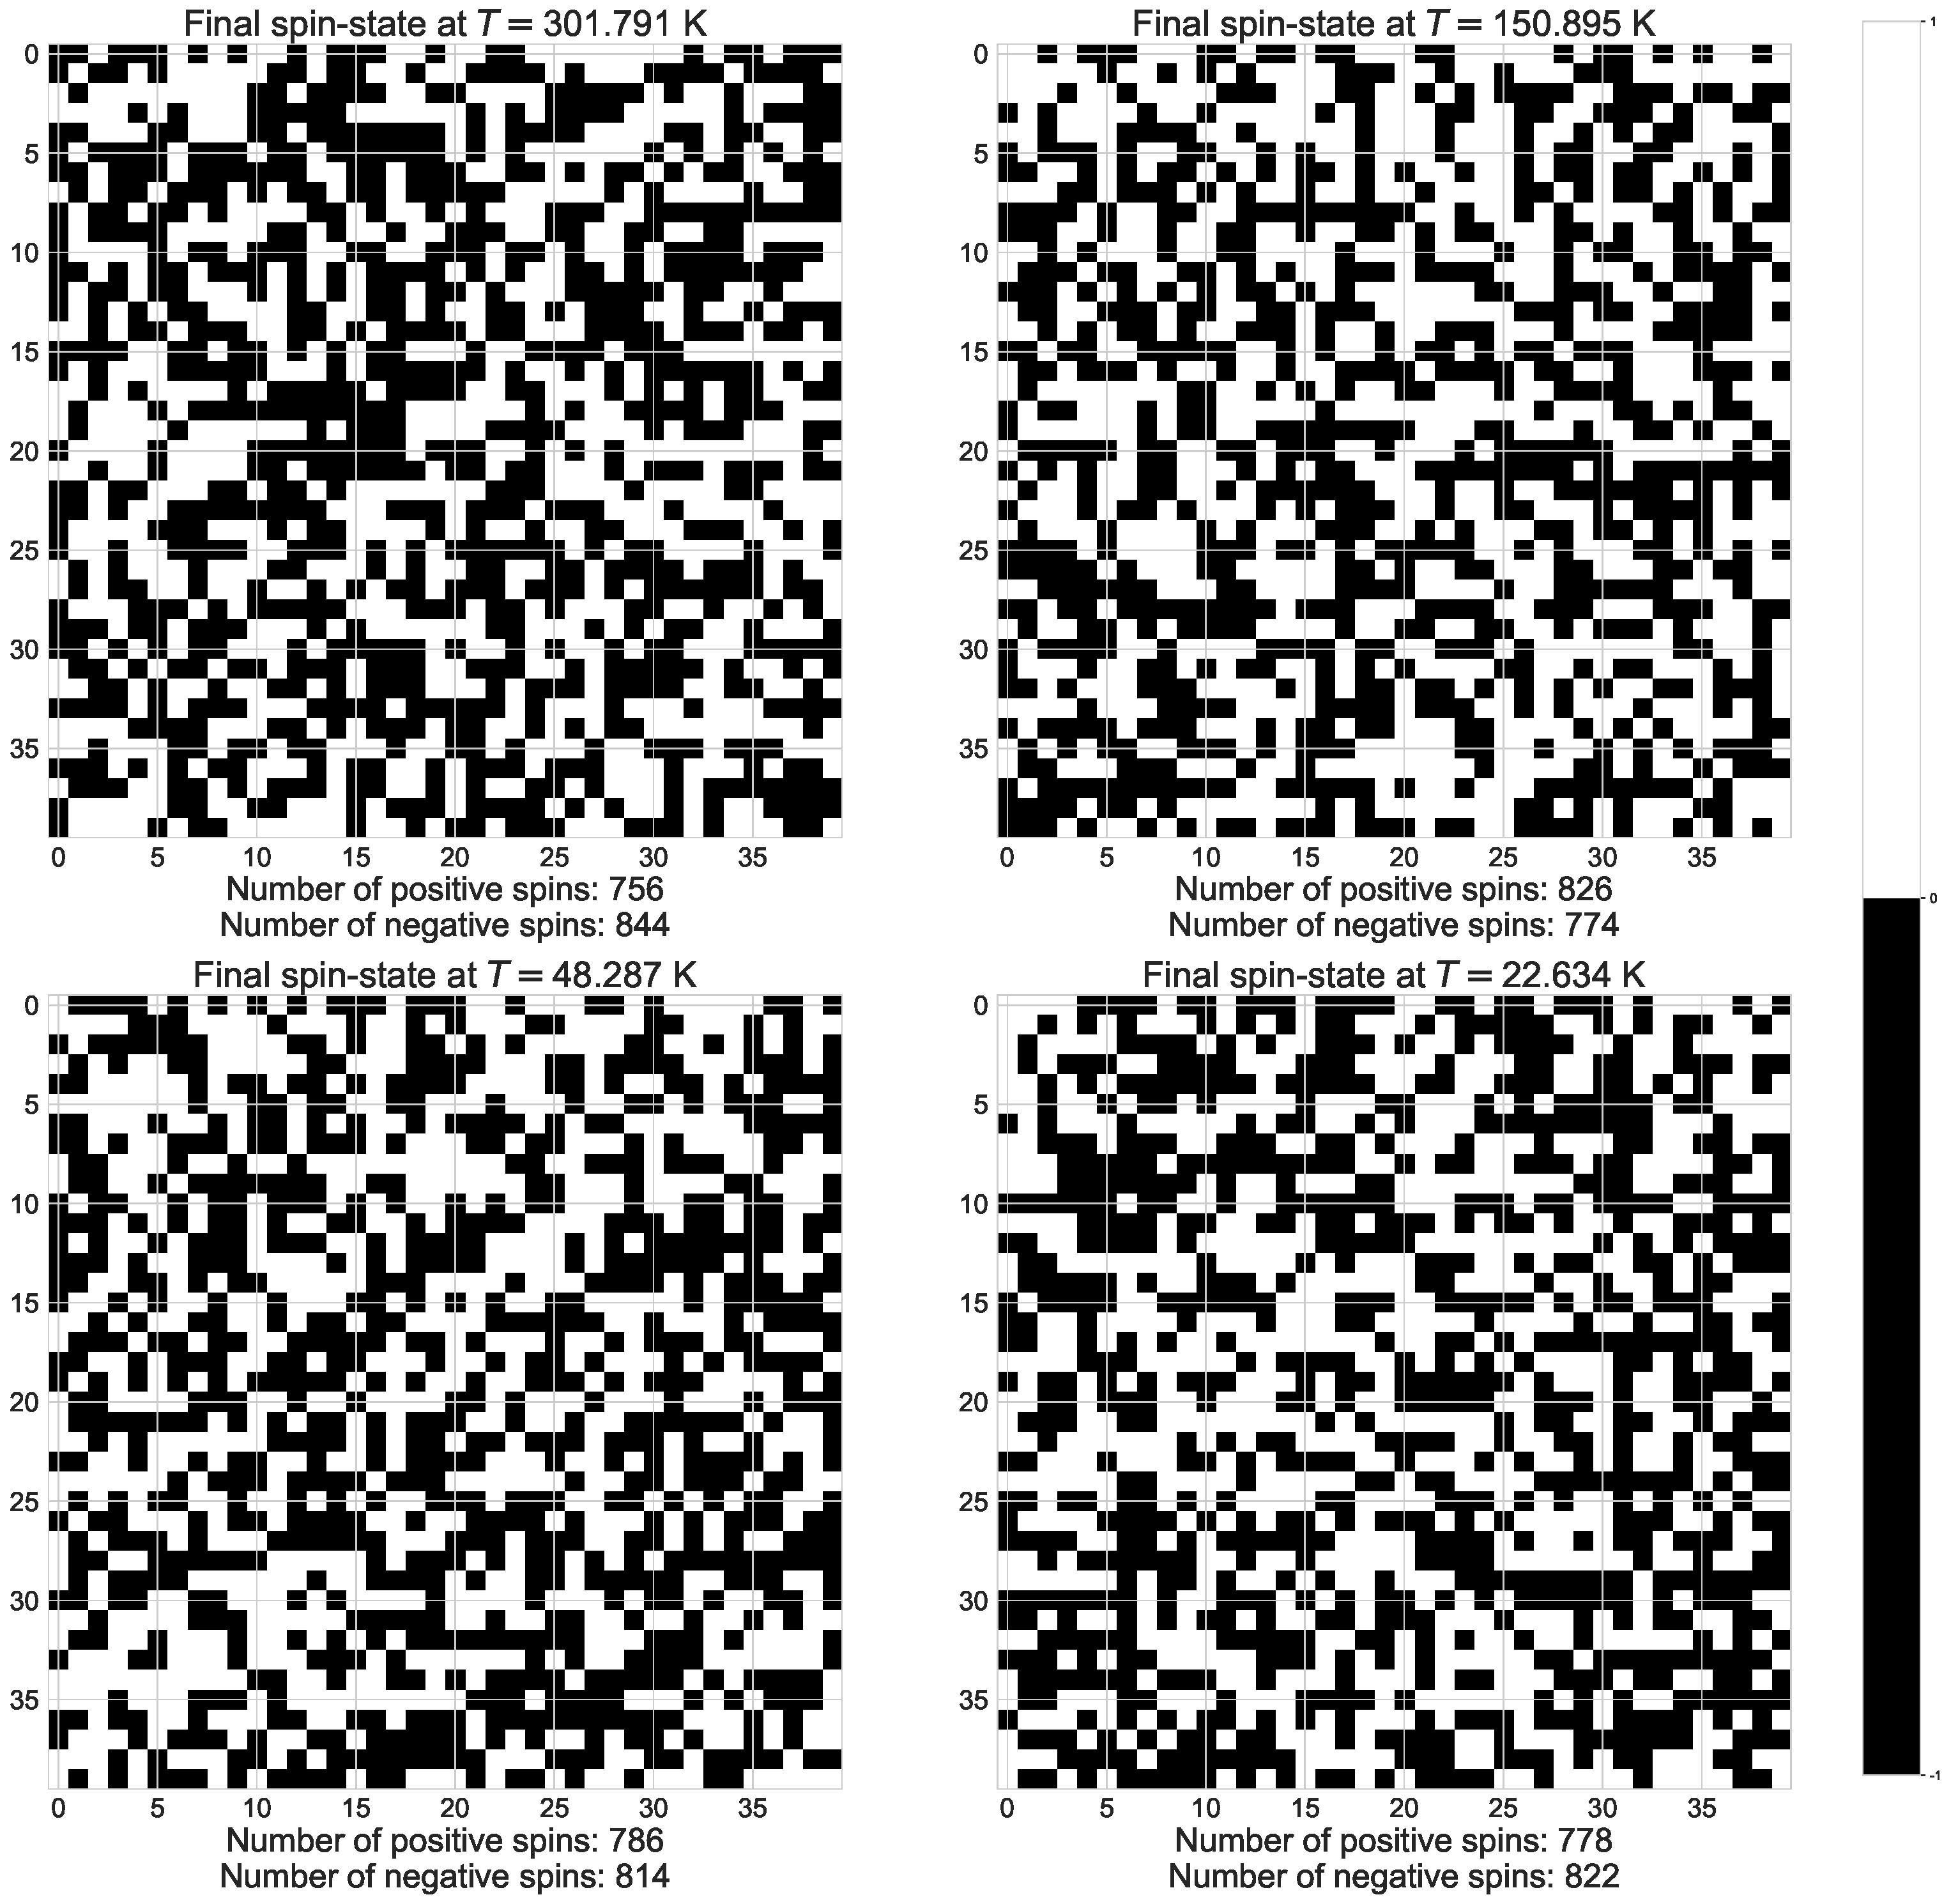
\includegraphics[width=\textwidth]{images/spin_states_2D.pdf}}
\captionof{figure}{A 2D Ising-modell végső állapota $N=100\,000$ lépés szimulálása után} \label{fig:10}
\newpage
{\centering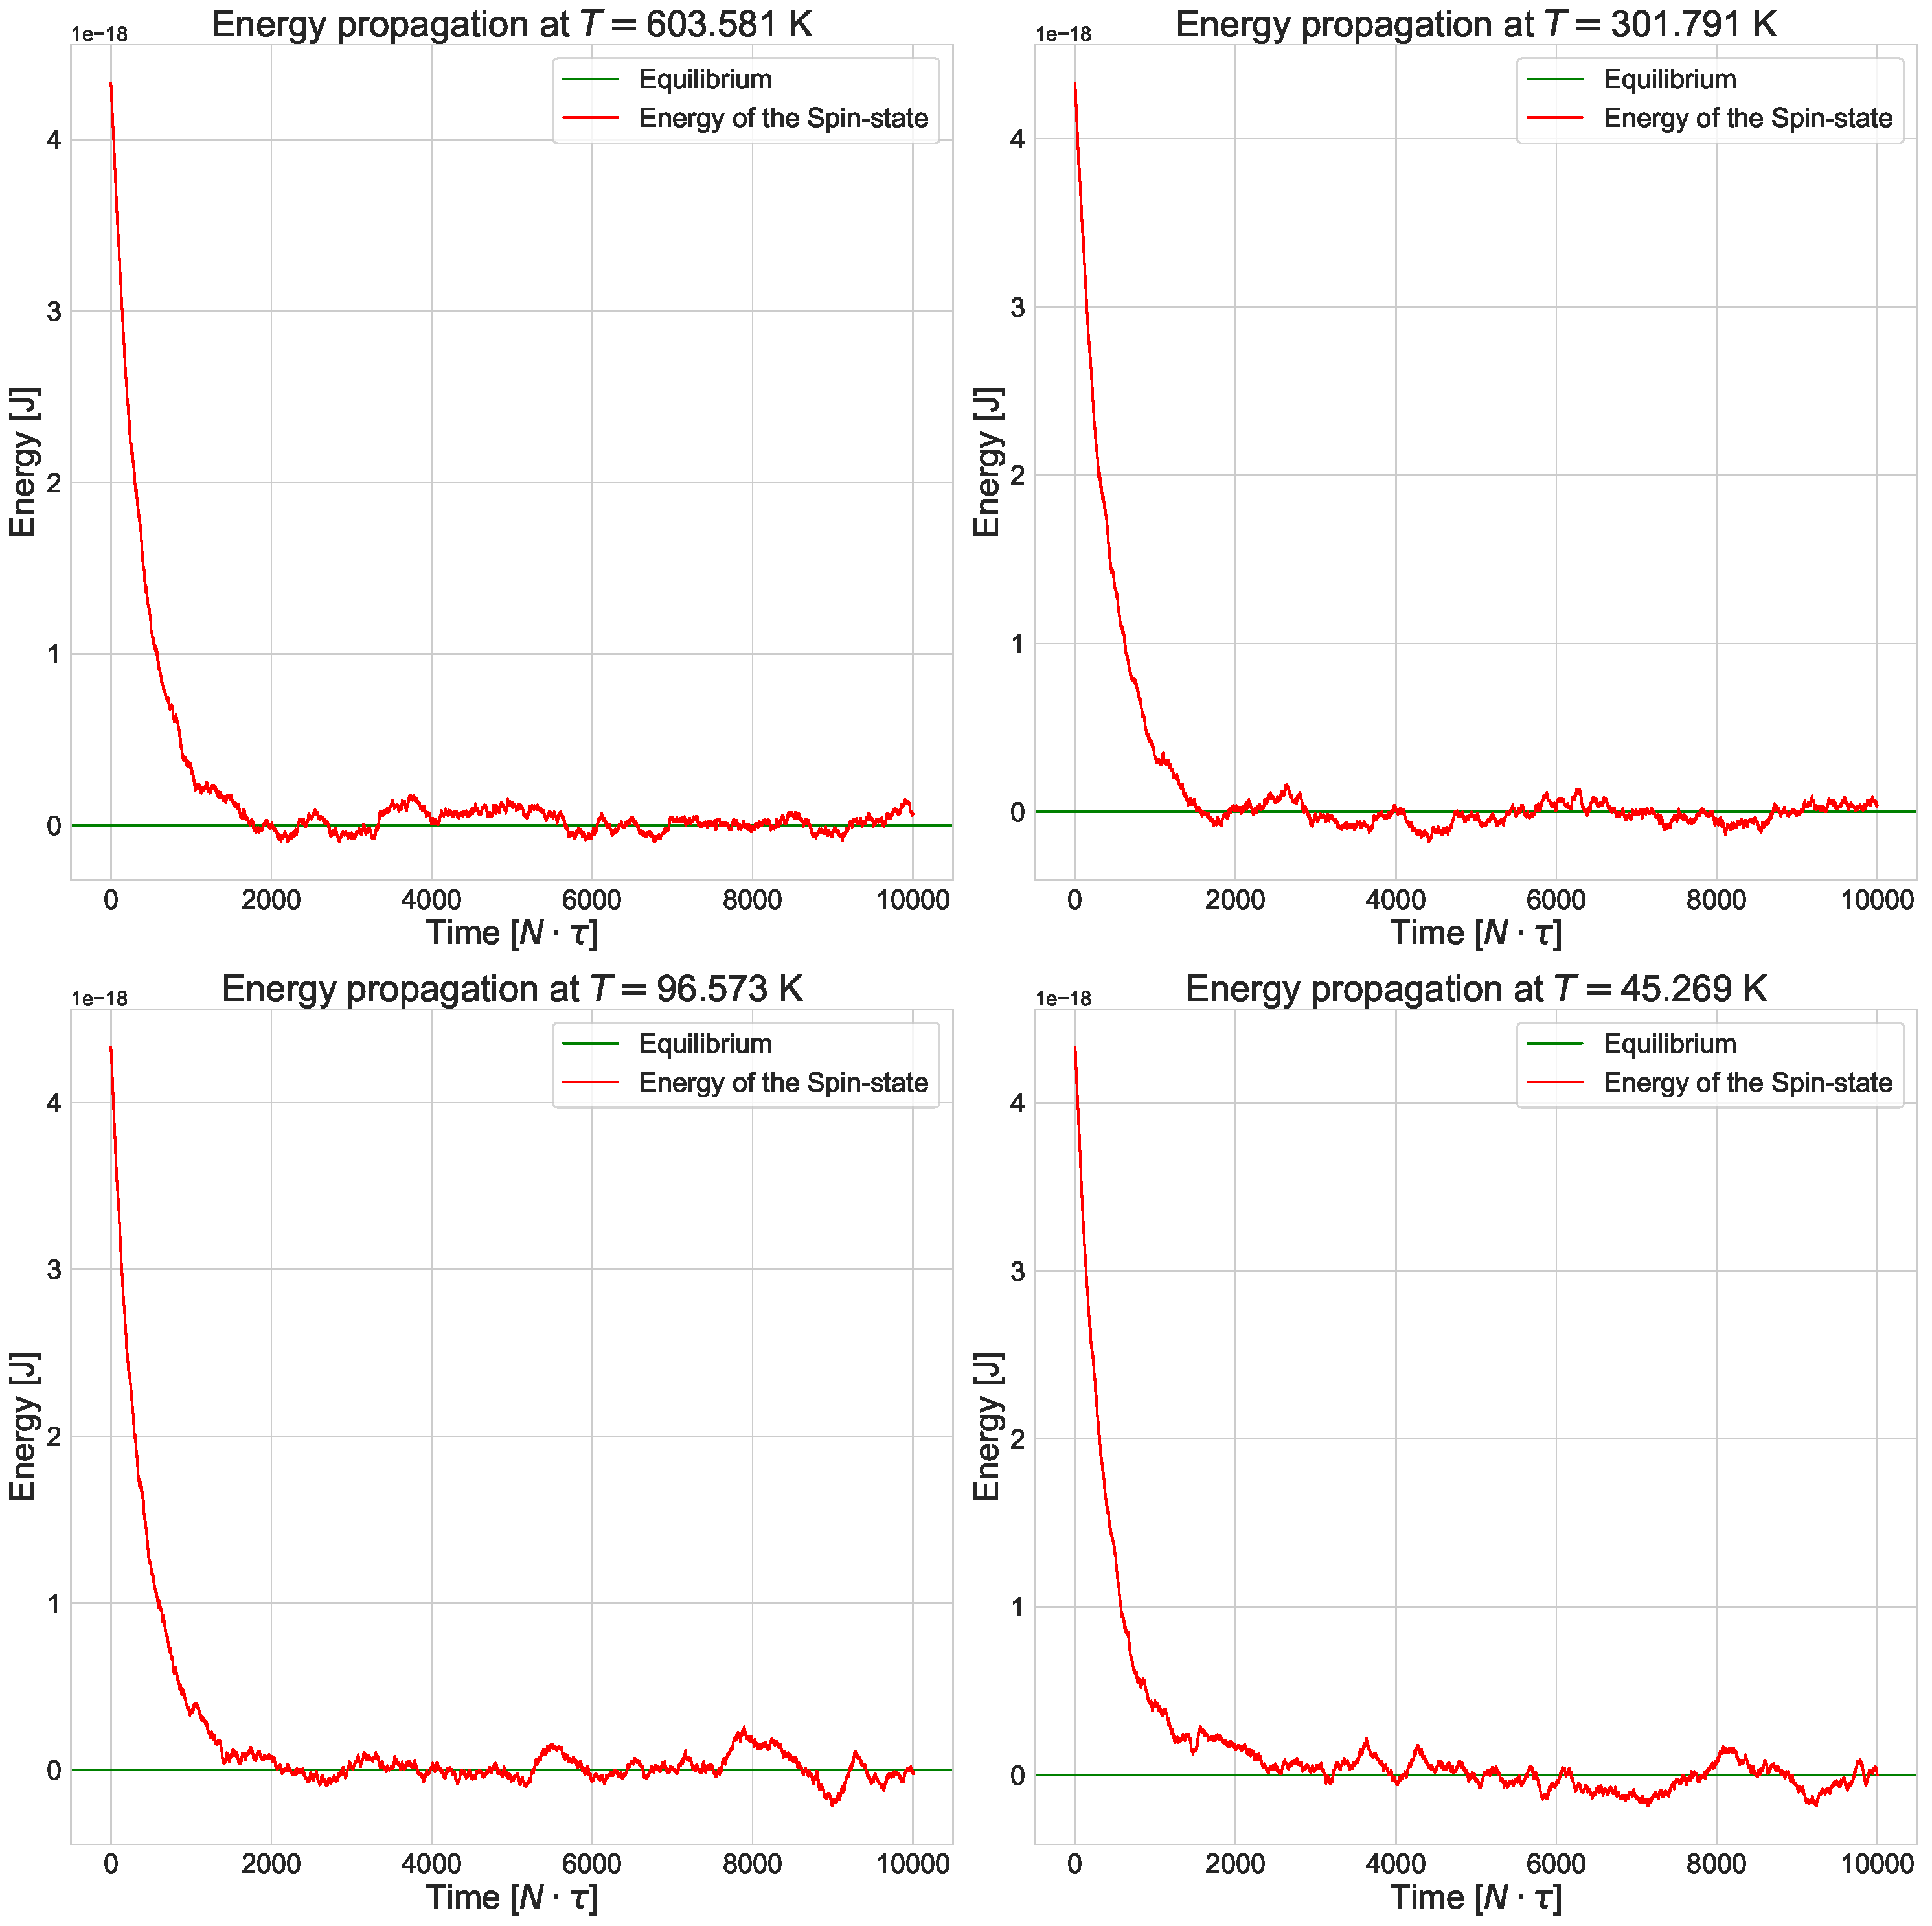
\includegraphics[width=\textwidth]{images/discrete_energies_2D.pdf}}
\captionof{figure}{A 2D Ising-modellben mérhető teljes energia időfejlődése} \label{fig:11}
\newpage
{\centering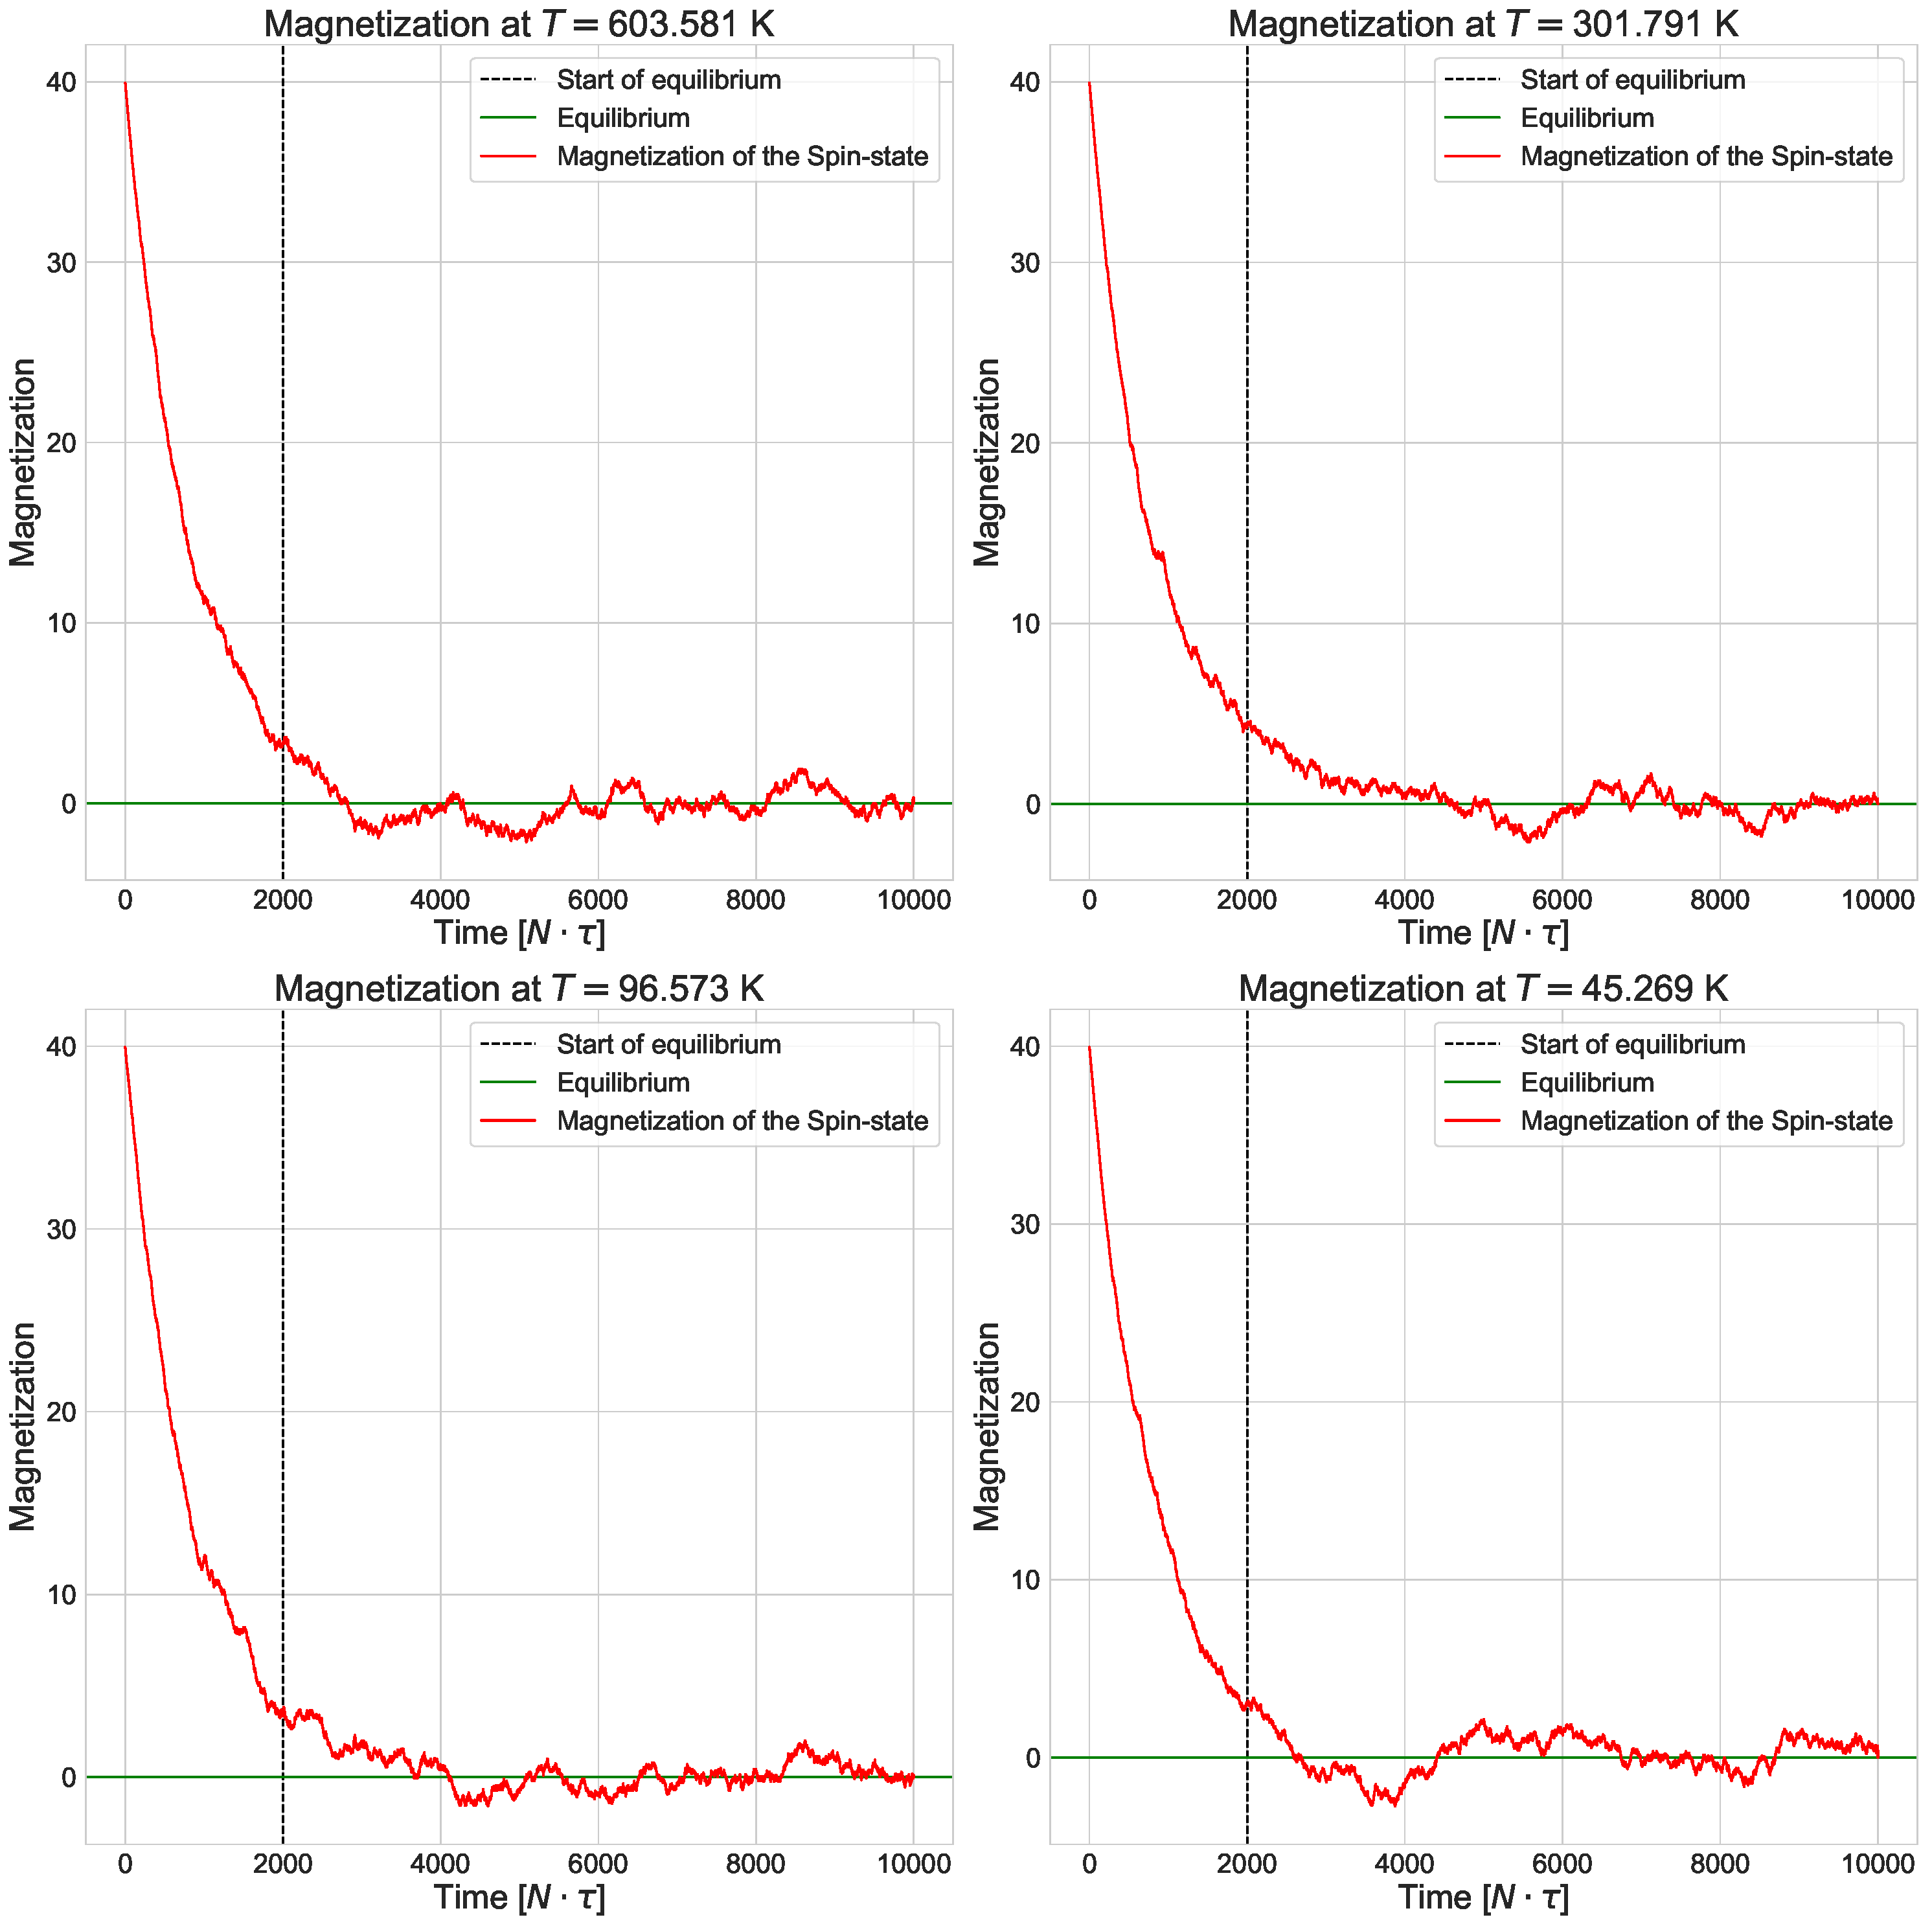
\includegraphics[width=\textwidth]{images/magnetization_2D.pdf}}
\captionof{figure}{A 2D Ising-modellben mérhető mágnesezettség időfejlődése} \label{fig:12}
\newpage
{\centering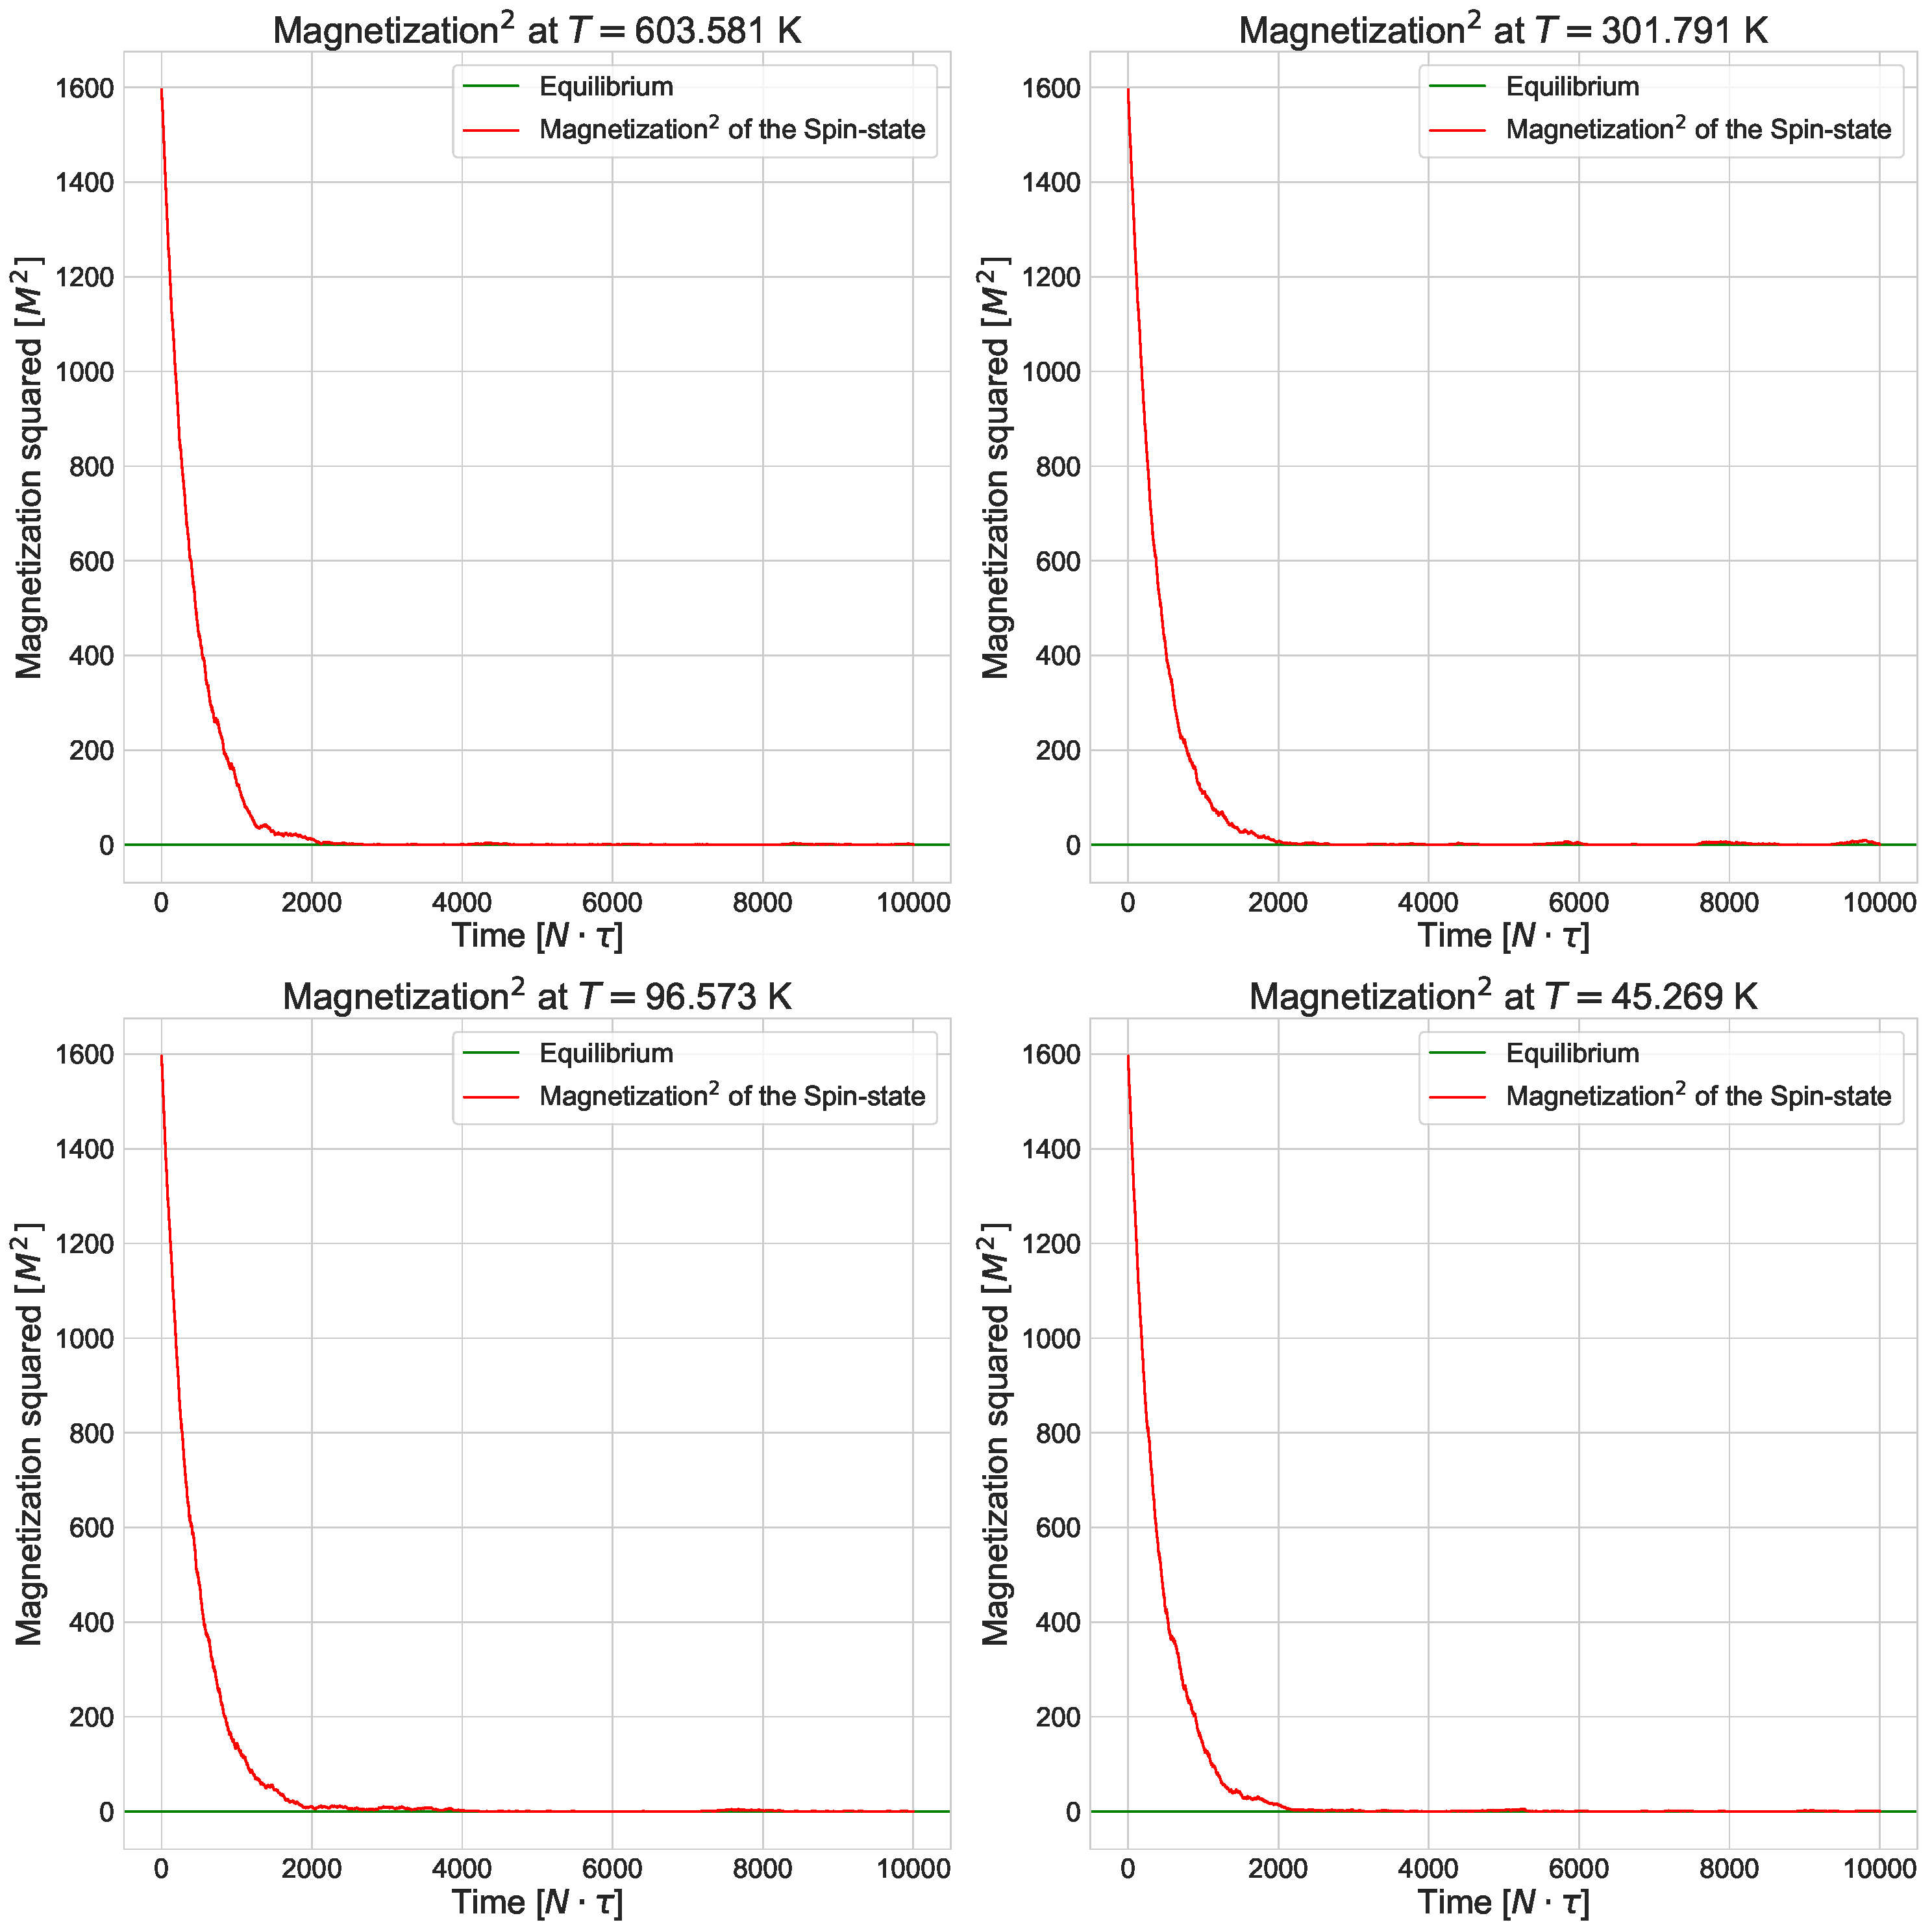
\includegraphics[width=\textwidth]{images/magnetization_squared_2D.pdf}}
\captionof{figure}{A 2D Ising-modellben mérhető mágnesezettség négyzetének időfejlődése} \label{fig:11}
\newpage
{\centering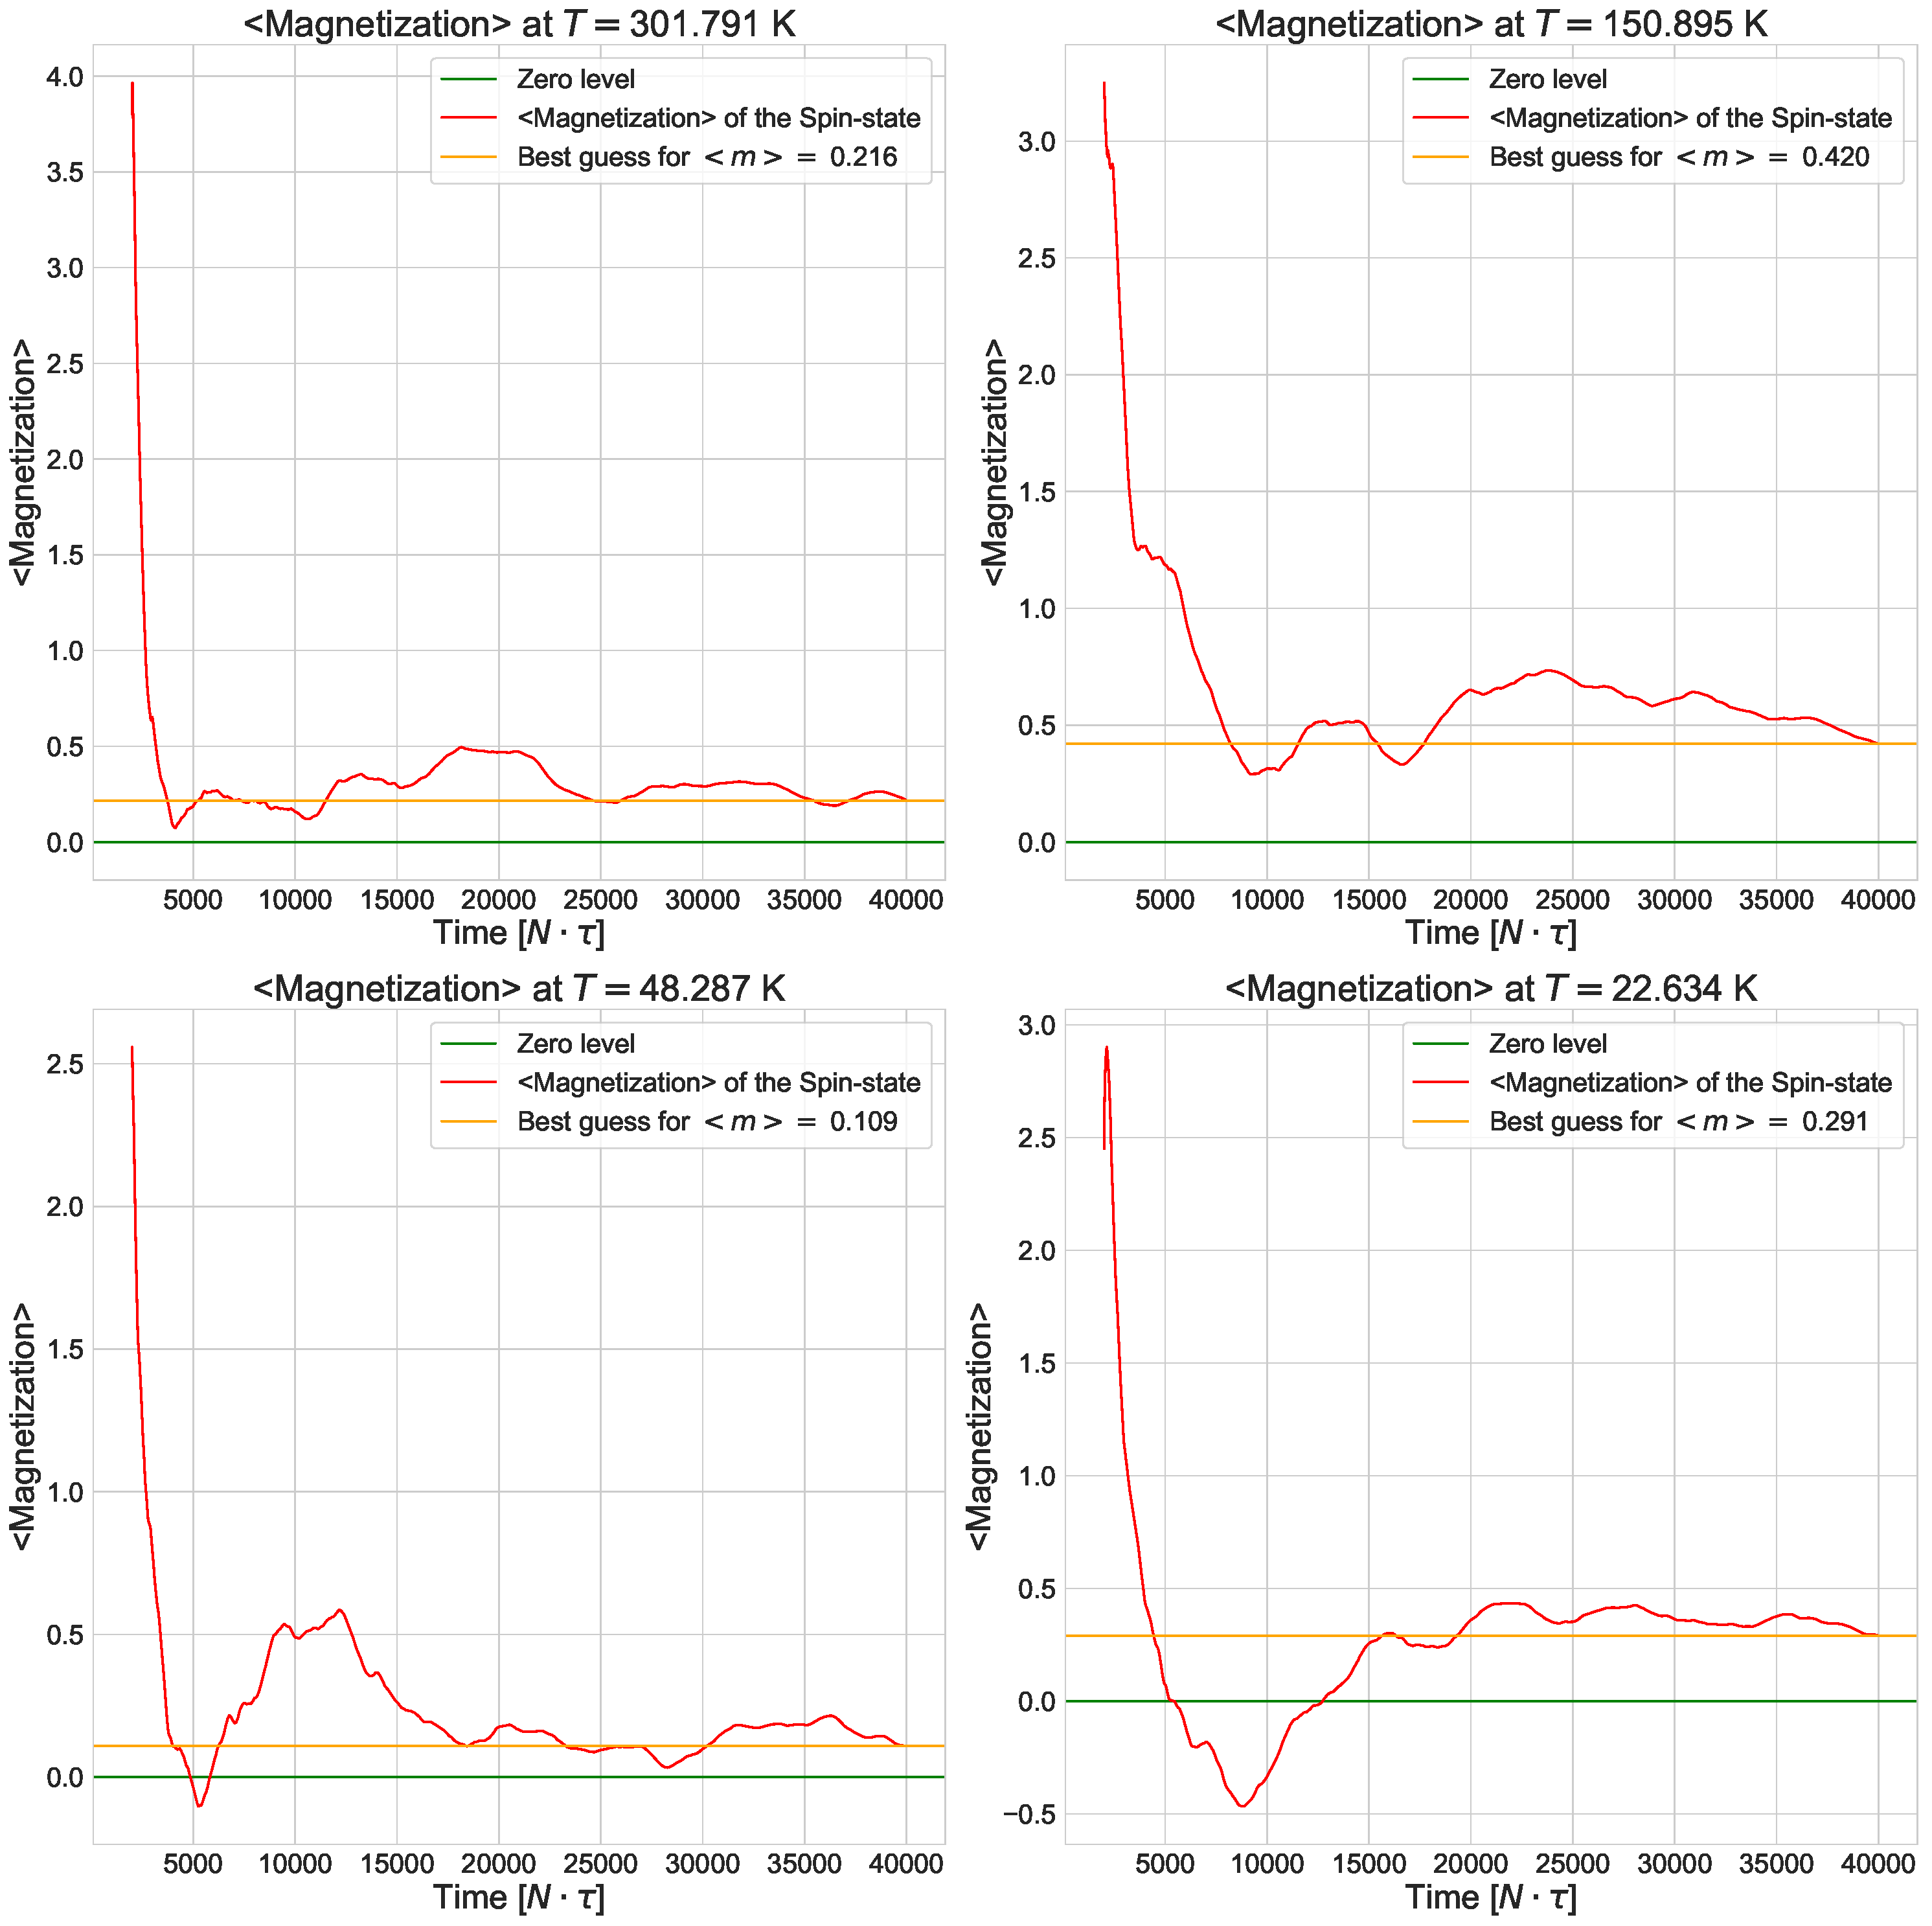
\includegraphics[width=\textwidth]{images/magnetization_mean_2D_off2000.pdf}}
\captionof{figure}{Az 2D Ising-modellben az egyensúlyi helyzet beállta után mérhető mágnesezettség időátlaga} \label{fig:12}
\newpage
{\centering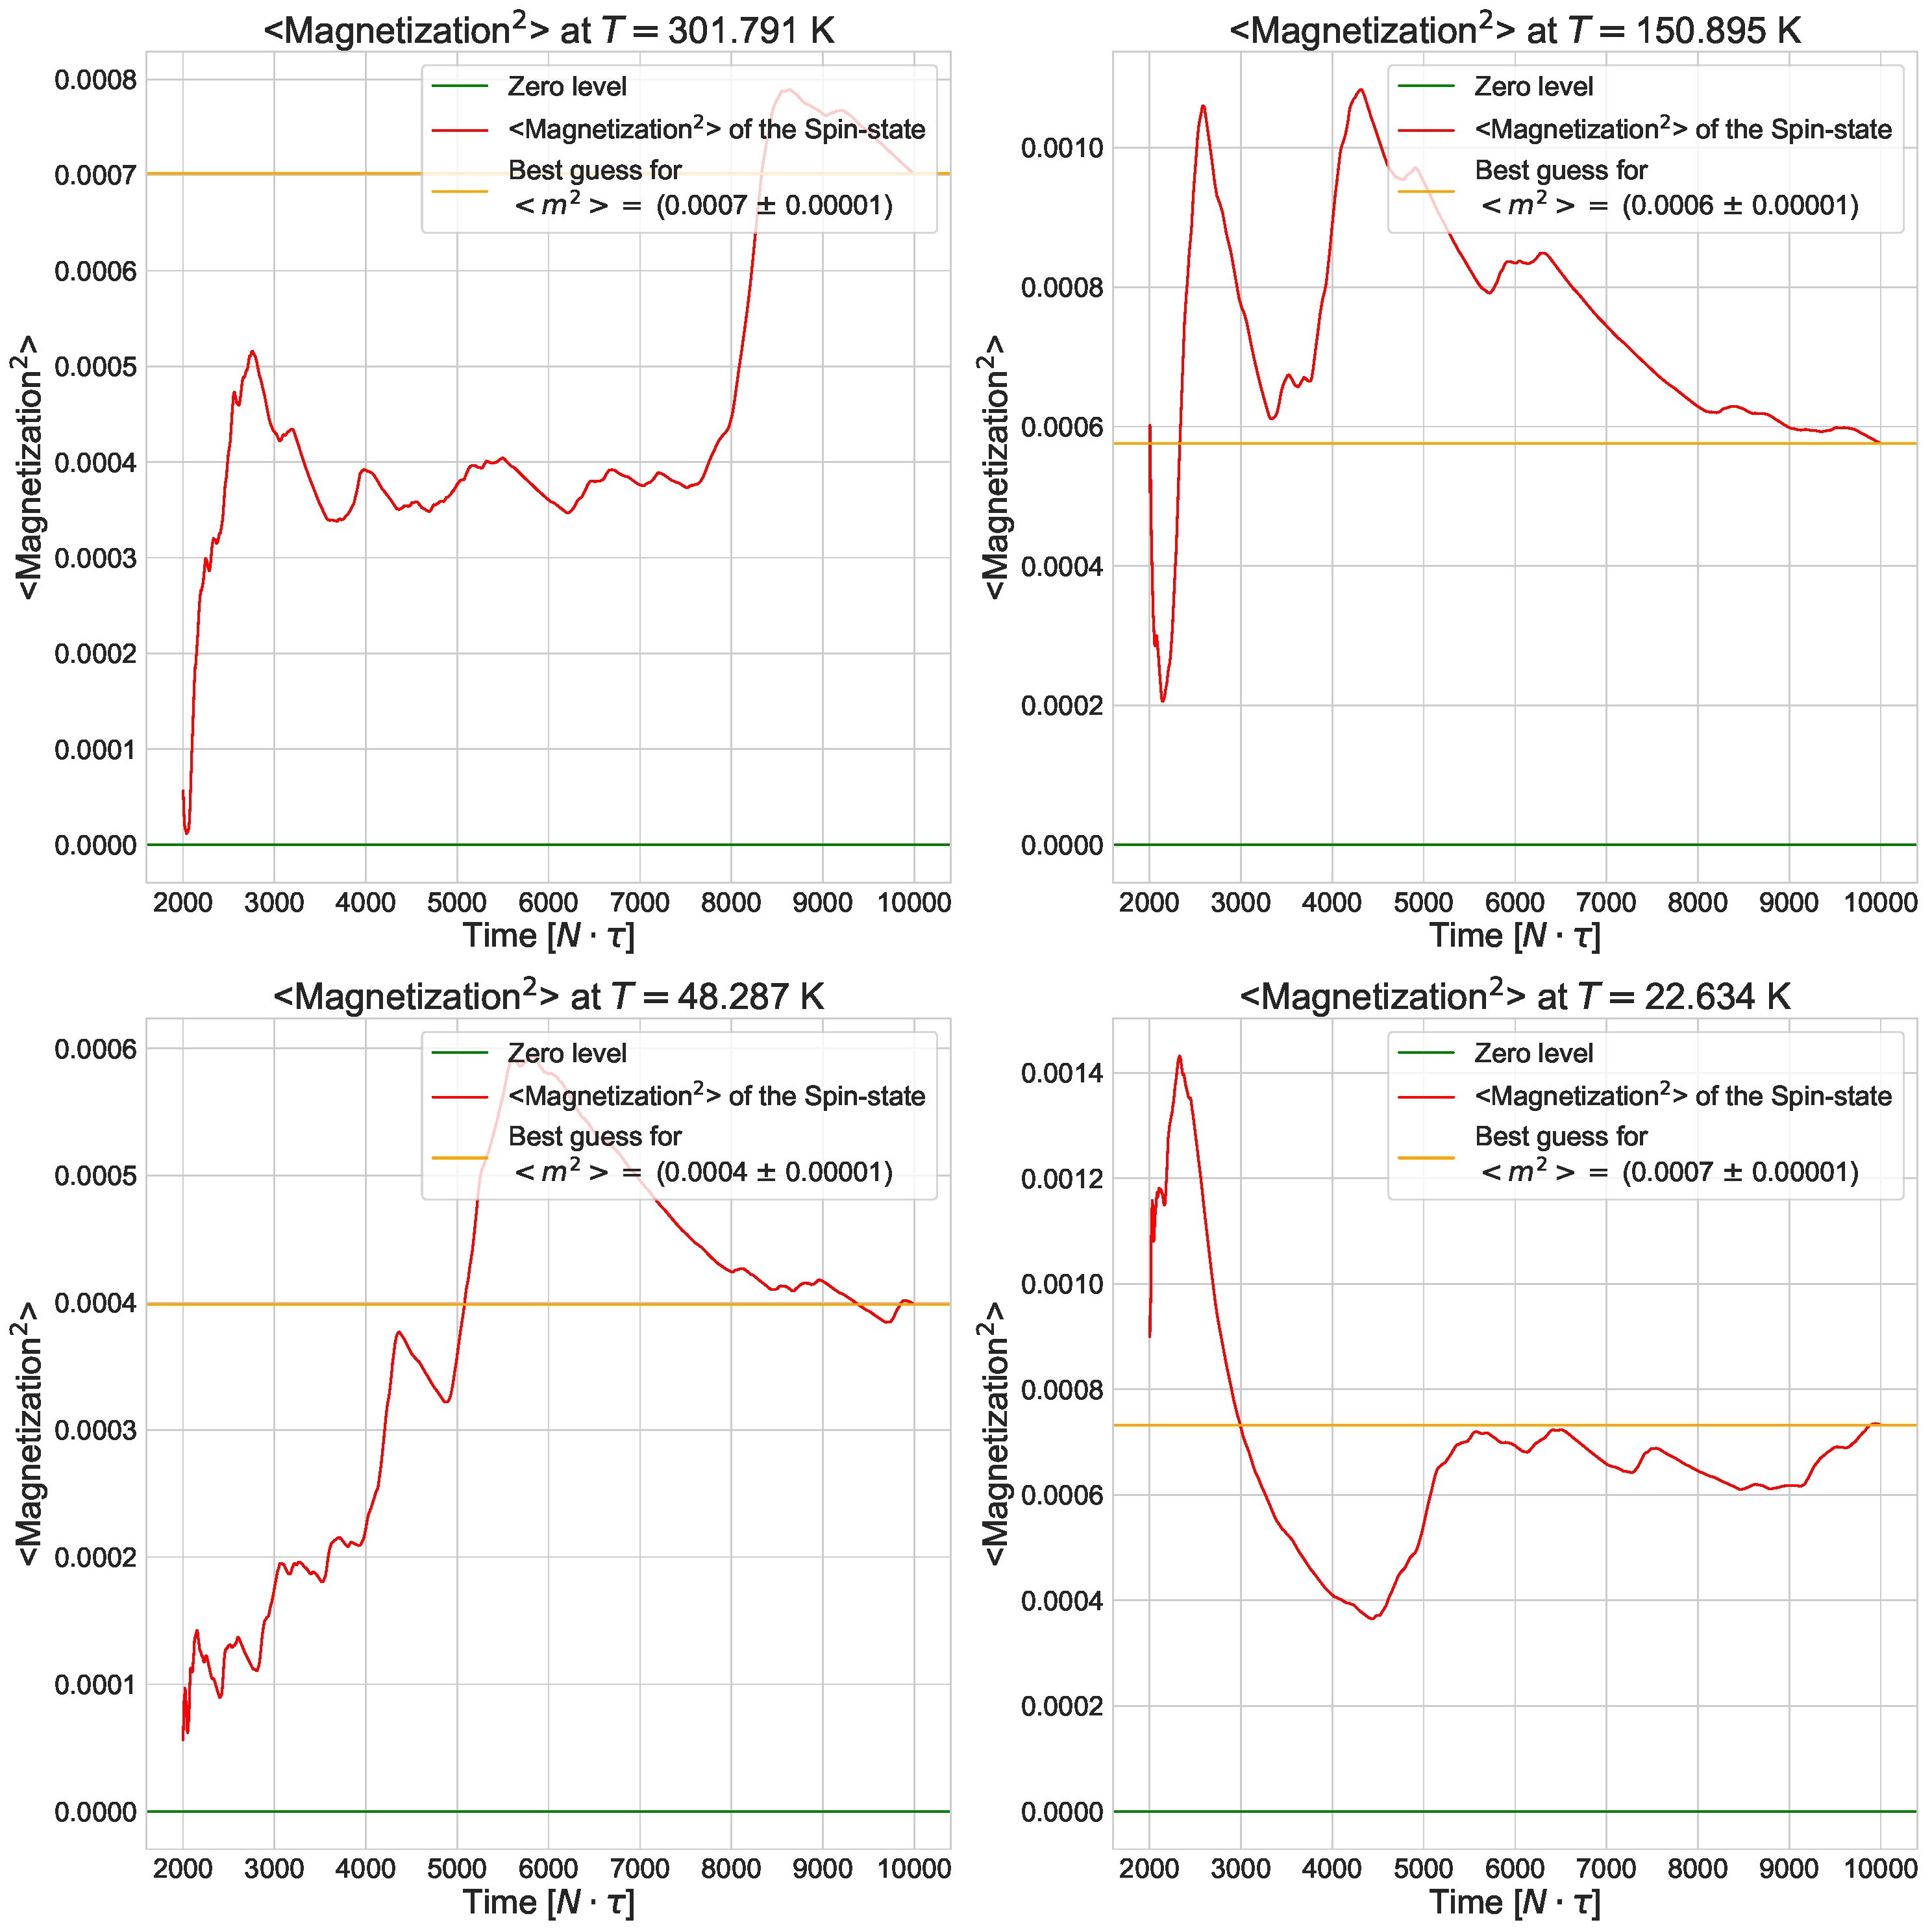
\includegraphics[width=\textwidth]{images/magnetization_squared_mean_2D_off2000.pdf}}
\captionof{figure}{Az 2D Ising-modellben az egyensúlyi helyzet beállta után mérhető mágnesezettség négyzetének időátlaga} \label{fig:13}
\newpage
{\centering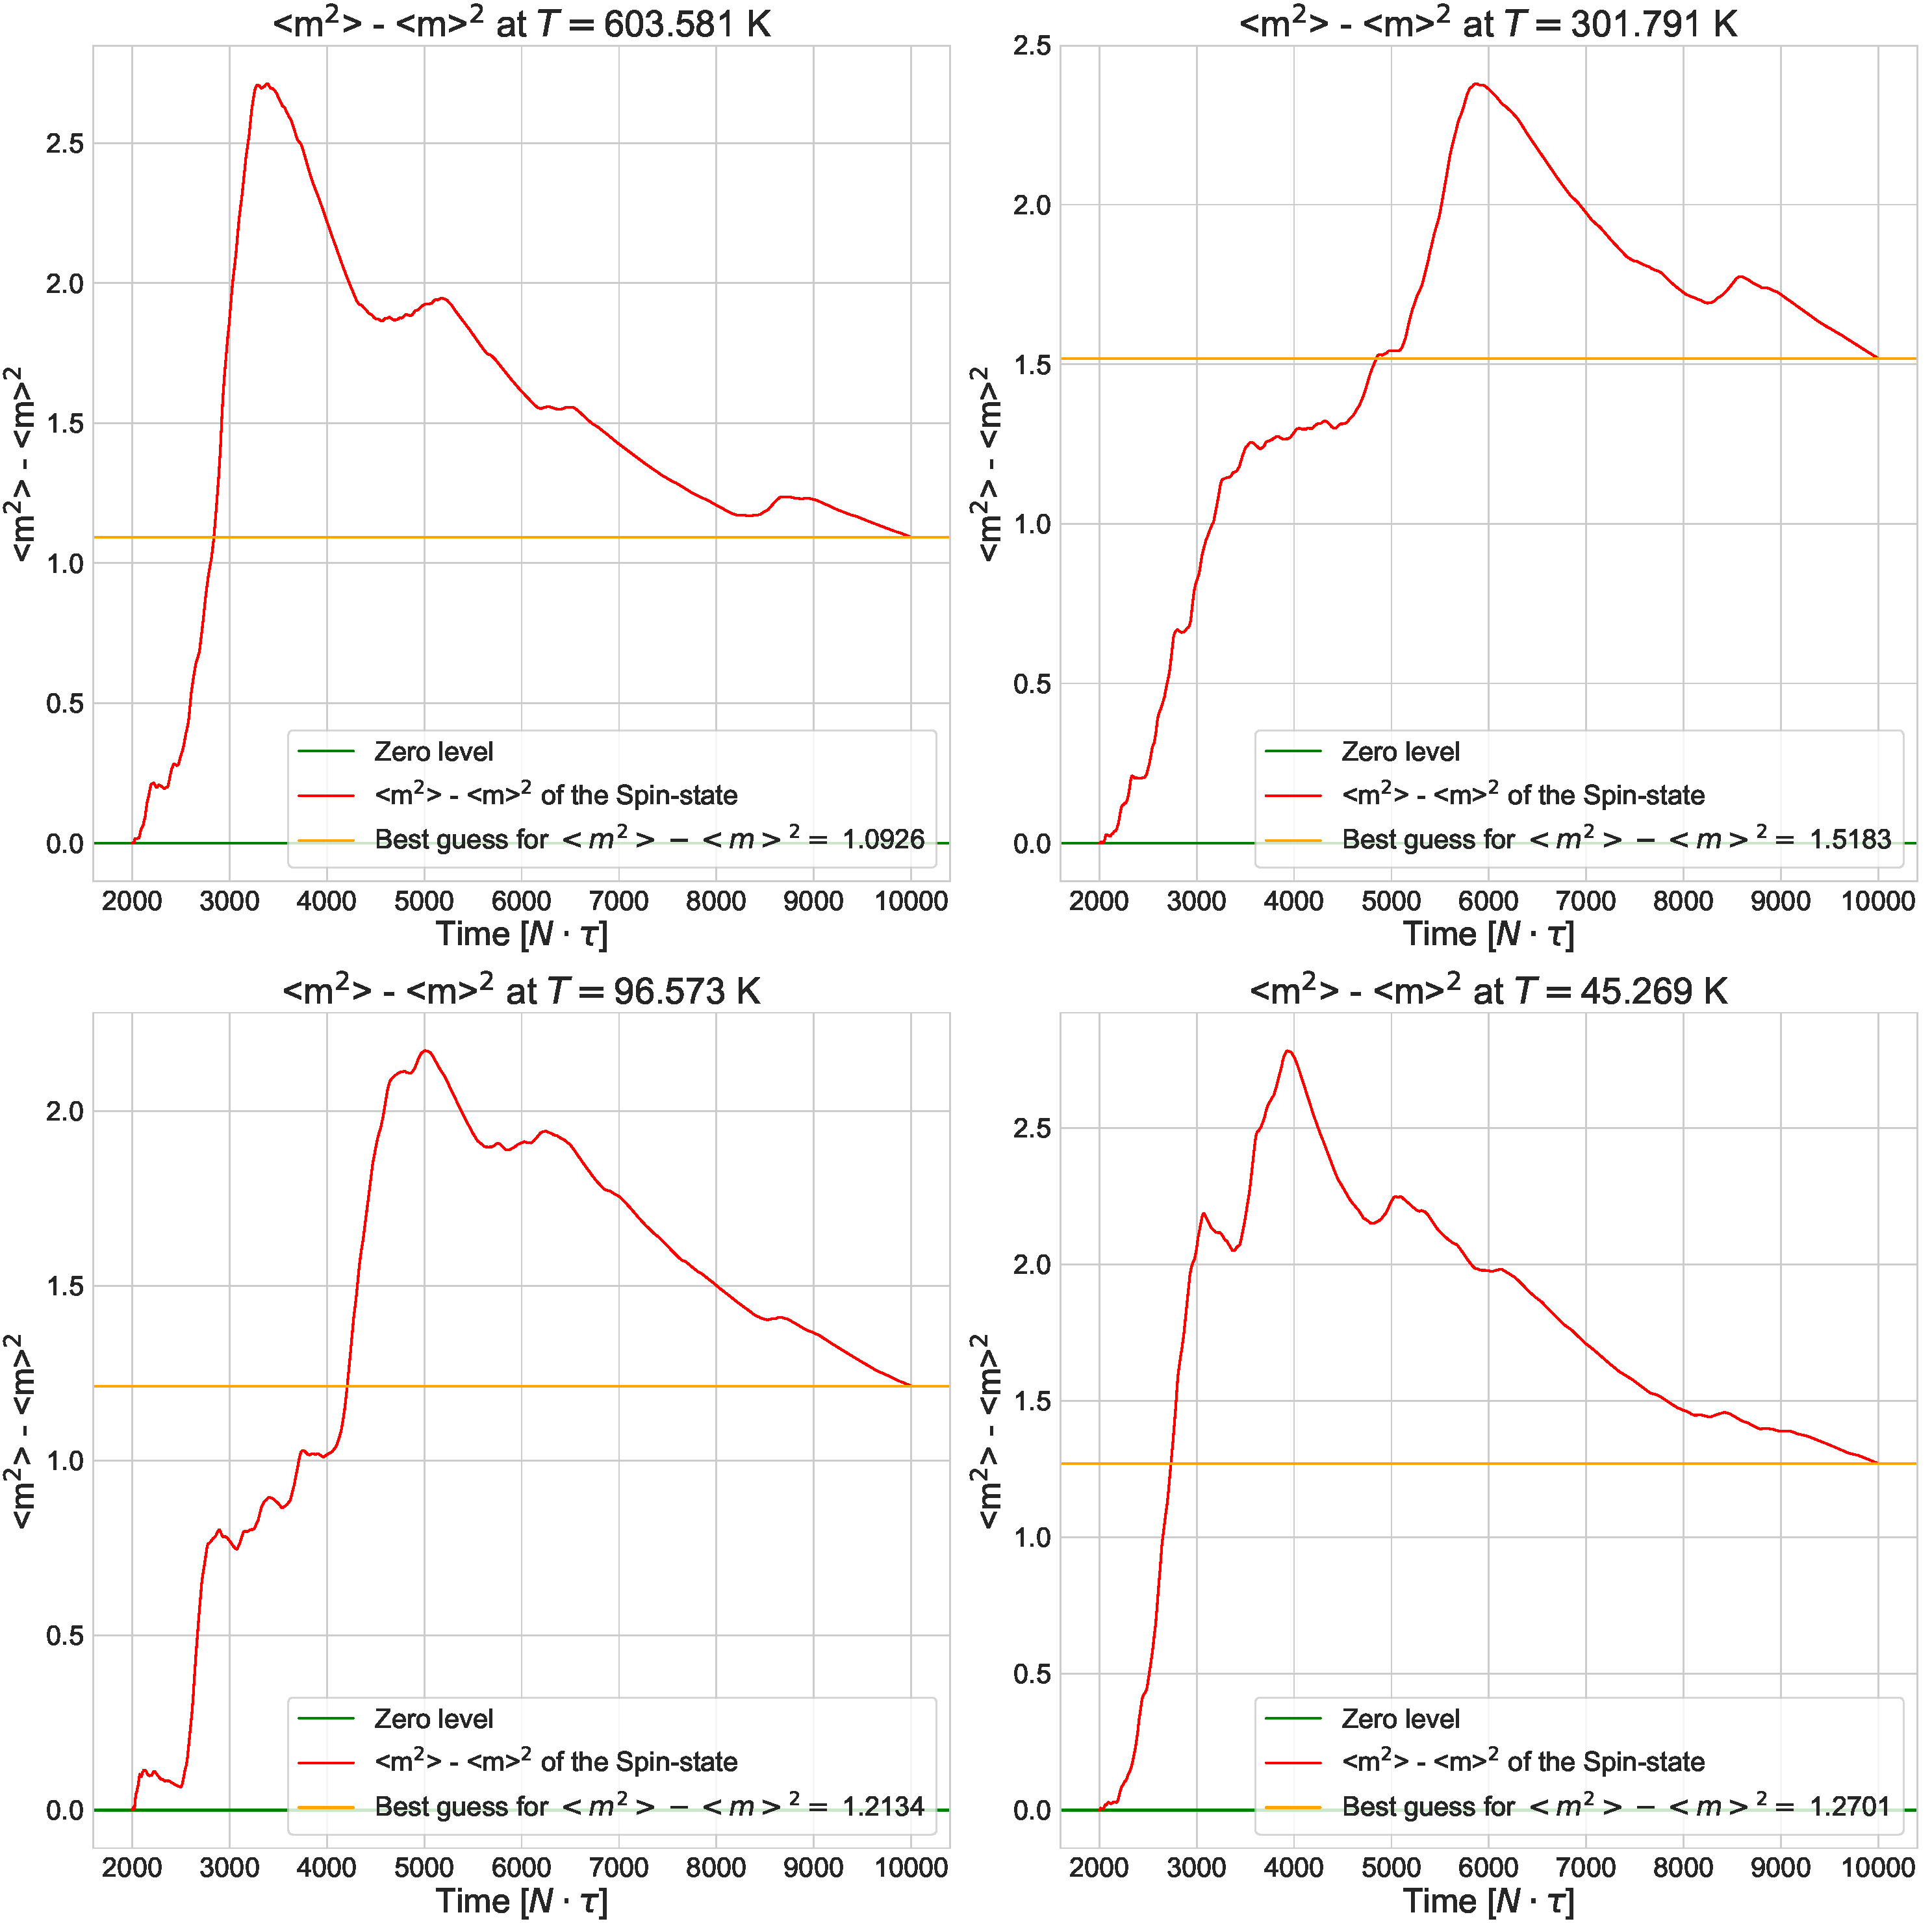
\includegraphics[width=\textwidth]{images/magnetization_diff_mean_2D_off2000.pdf}}
\captionof{figure}{Az 2D Ising-modellben az egyensúlyi helyzet beállta után mérhető $\left< m^{2} \right> - \left< m \right>^{2}$ mennyiség időátlaga} \label{fig:14}